
%
\section{Results} % (fold)
\label{sec:tcl_results}
%
We applied our algorithm to stress tensor fields obtained from structural
mechanics simulations of varying complexity.
%
The Cauchy stress tensor (often referred to as $\mathbf{\sigma}$ in mechanics
literature) is a symmetric tensor that desribes the local stress state of an
object experiencing small elastic deformations.
%
Its eigenvectors point in the directions of the principal stresses.
%
The sign of the eigenvalues indicate if the stress is compressive or tensile.
%
Swirling structures in stress tensor fields can result from torque induced in
part of a structure.
%
As we will show, it is not always intuitive where this will happen in a complex
structure subject to a load or deformation.
%
Computing tensor core lines allows an easy identification of these phenomena.
%
In this section, we present the results of our algorithm on several datasets, we
analyze its performance and parameter sensitivity, and we compare our results to
the toplogical skeleton formed by degenerate lines.
%
\paragraph*{Cylinder} % (fold)
\label{sub:torque_applied_to_a_cylinder}
%
In \autoref{fig:tube_lines} we show the eigenvector trajectories resulting from
applying a torque around the long axis of a cylinder.
%
The yellow line visible in the center is the result of our algorithm applied to
this case after filtering out numerically unstable solutions.
%
These solutions occur because the third eigenvector, which is orthogonal to the
other two, points outwards from the center line everywhere in the domain.
%
This means that the trajectories of this eigenvector are straight lines
everywhere inside the cylinder.
%
Situations like this are common in stress tensor fields, and are handled in our
algorithm by the threshold $M$.
%
Nevertheless, single line segments with low numeric stability $s$ may occur due
to noise (see \autoref{fig:unfiltered_lines}).
%
After filtering them out, the clear central line visible in
\autoref{fig:tube_lines} remains.
%
% subsection torque_applied_to_a_cylinder (end)
%
\paragraph*{Handle} % (fold)
\label{sub:hook}
%
\begin{figure*}
    \centering
    \setlength\figurewidth\linewidth
    %
%
\pgfplotsset{colormap={cubicyf}{
rgb = (0.5151, 0.0482, 0.66969999999999996)
rgb = (0.52071100000000003, 0.16895499999999999, 0.80057400000000001)
rgb = (0.49369400000000002, 0.27859600000000001, 0.91182399999999997)
rgb = (0.44002599999999997, 0.369475, 0.98497800000000002)
rgb = (0.39893200000000001, 0.45759300000000003, 0.98705299999999996)
rgb = (0.35065099999999999, 0.54064400000000001, 0.92960799999999999)
rgb = (0.29882700000000001, 0.61562499999999998, 0.85772899999999996)
rgb = (0.239928, 0.68506100000000003, 0.76953099999999997)
rgb = (0.22883200000000001, 0.73934900000000003, 0.67328699999999997)
rgb = (0.263297, 0.78608, 0.56998800000000005)
rgb = (0.29810700000000001, 0.82833699999999999, 0.46021400000000001)
rgb = (0.33091999999999999, 0.86407100000000003, 0.35267399999999999)
rgb = (0.38306000000000001, 0.898169, 0.28730899999999998)
rgb = (0.49023, 0.91748099999999999, 0.30796099999999998)
rgb = (0.62372000000000005, 0.92602600000000002, 0.33230900000000002)
rgb = (0.71745800000000004, 0.92527000000000004, 0.342476)
rgb = (0.80000000000000004, 0.92549999999999999, 0.35289999999999999)
}}
\pgfplotsset{colormap={rdoryl}{
rgb(0)=(1, 1, 0.80000000000000004)
rgb(1)=(1, 0.96678200000000003, 0.71879999999999999)
rgb(2)=(1, 0.93134899999999998, 0.63218799999999997)
rgb(3)=(0.998139, 0.89219499999999996, 0.54929600000000001)
rgb(4)=(0.99617100000000003, 0.85282599999999997, 0.46662100000000001)
rgb(5)=(0.99607800000000002, 0.77780899999999997, 0.38394499999999998)
rgb(6)=(0.99607800000000002, 0.70103800000000005, 0.30126900000000001)
rgb(7)=(0.99418700000000004, 0.62805100000000003, 0.26777400000000001)
rgb(8)=(0.99221800000000004, 0.55521699999999996, 0.23627799999999999)
rgb(9)=(0.99024999999999996, 0.43280299999999999, 0.20096900000000001)
rgb(10)=(0.98828099999999997, 0.30878899999999998, 0.16553599999999999)
rgb(11)=(0.94017700000000004, 0.20592099999999999, 0.137793)
rgb(12)=(0.89096500000000001, 0.10356, 0.110235)
rgb(13)=(0.81656300000000004, 0.051580000000000001, 0.12918099999999999)
rgb(14)=(0.741761, 0.00040000000000000002, 0.148866)
rgb(15)=(0.62203799999999998, 0, 0.14902000000000001)
rgb(16)=(0.50196099999999999, 0, 0.14902000000000001)
}}
%
\begin{tikzpicture}[
    font=\small
]
    \tikzstyle{image} = [inner sep=0, outer sep=0, node distance = 0.25cm and 0.25cm]

    % place image in node
    \node[image] (image1)
    {
        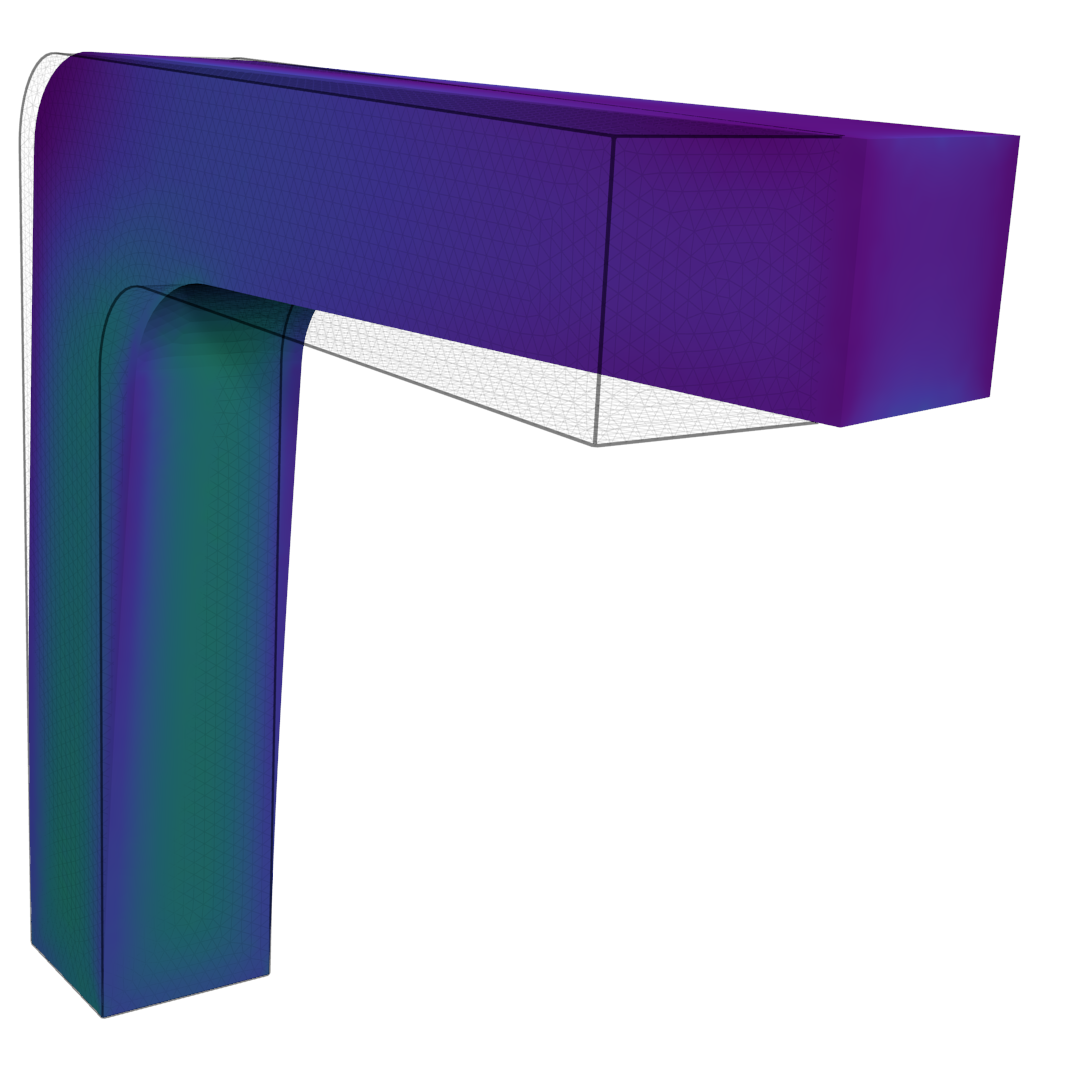
\includegraphics[width=0.305\figurewidth]{figures/hook2_deformation}%
    };

    \node[image, below=of image1] (image2)
    {
        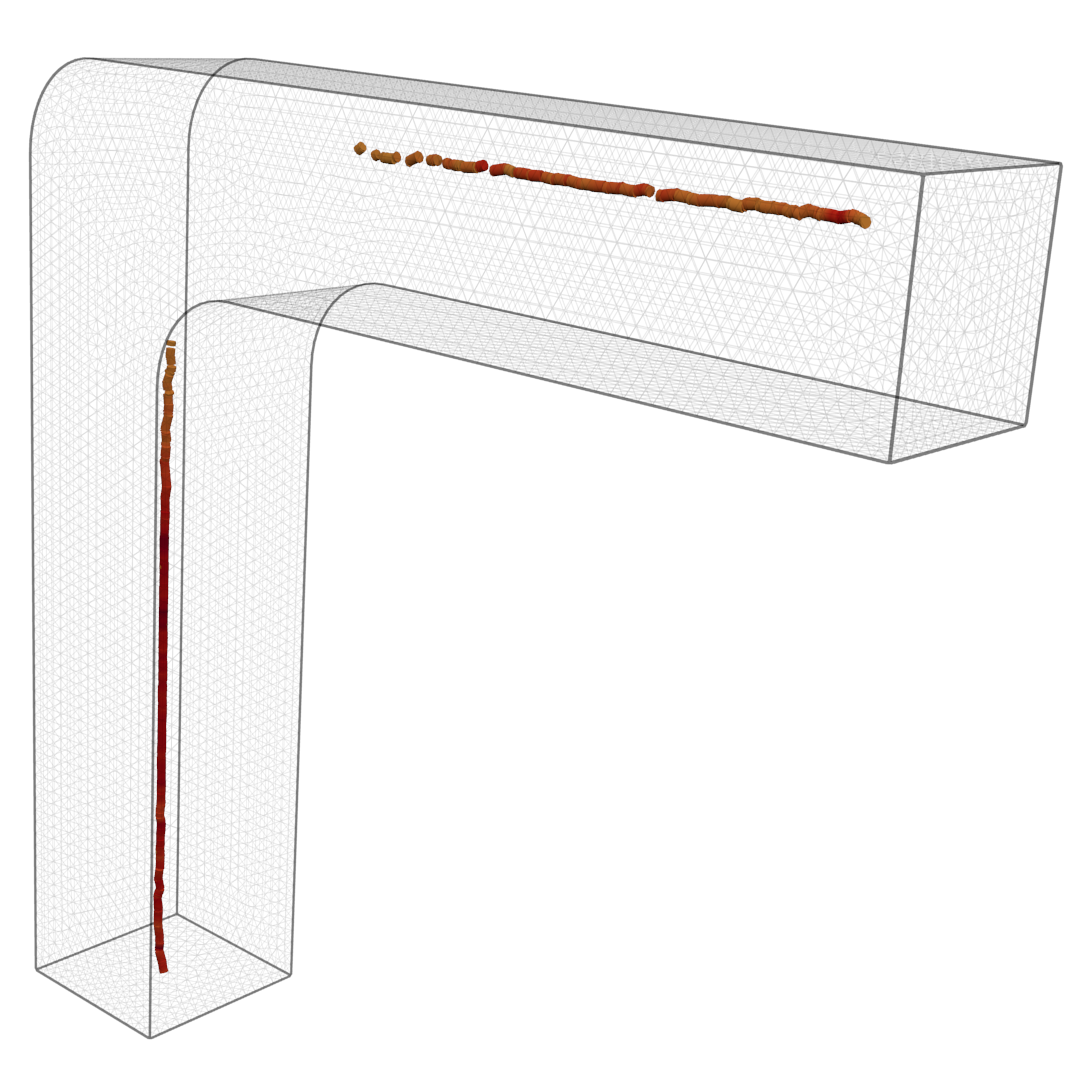
\includegraphics[width=0.305\figurewidth]{figures/hook2_lines}%
    };

    \node[image, below=of image2] (image3)
    {
        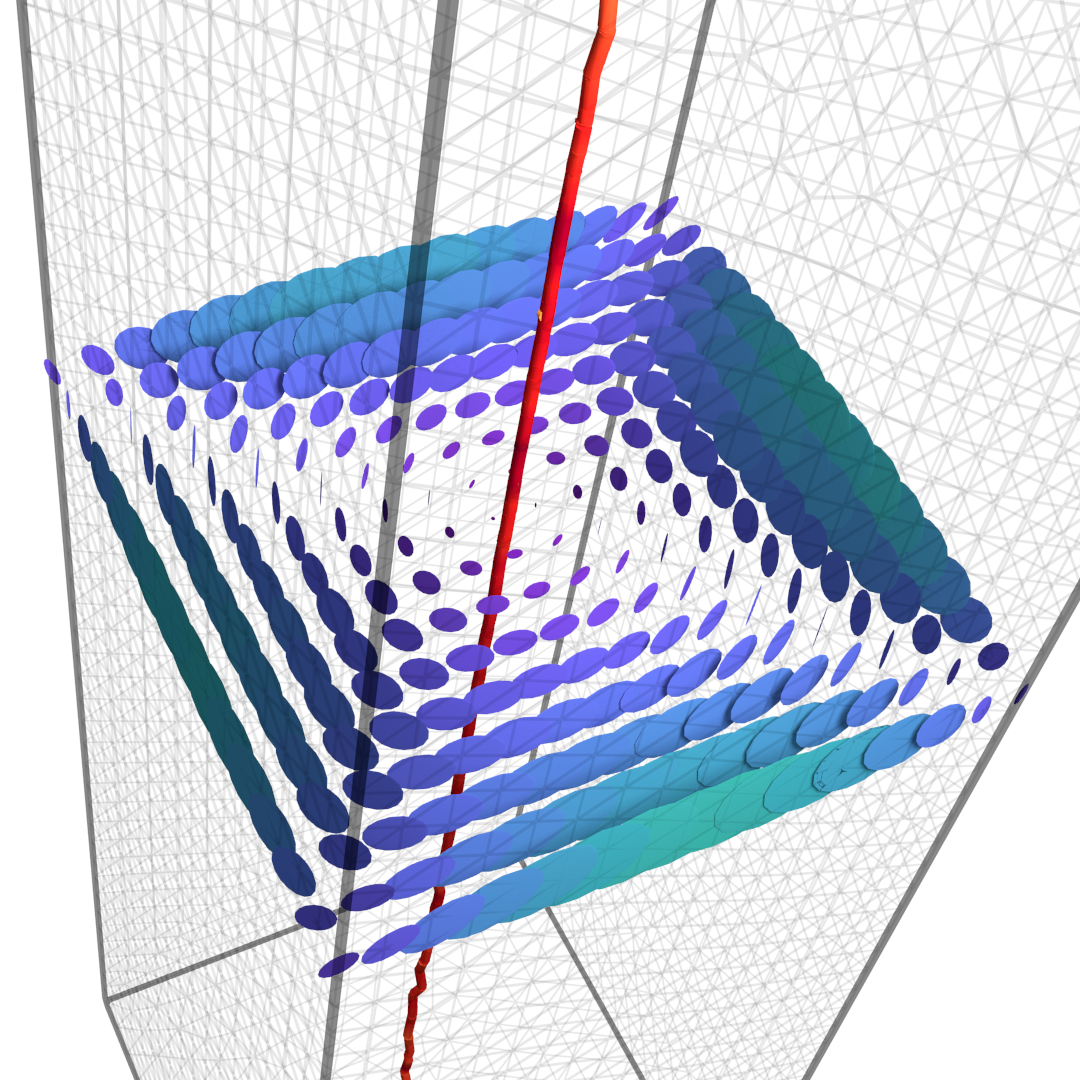
\includegraphics[width=0.305\figurewidth]{figures/hook2_detail1}%
    };

    \node[image, below=of image3] (image4)
    {
        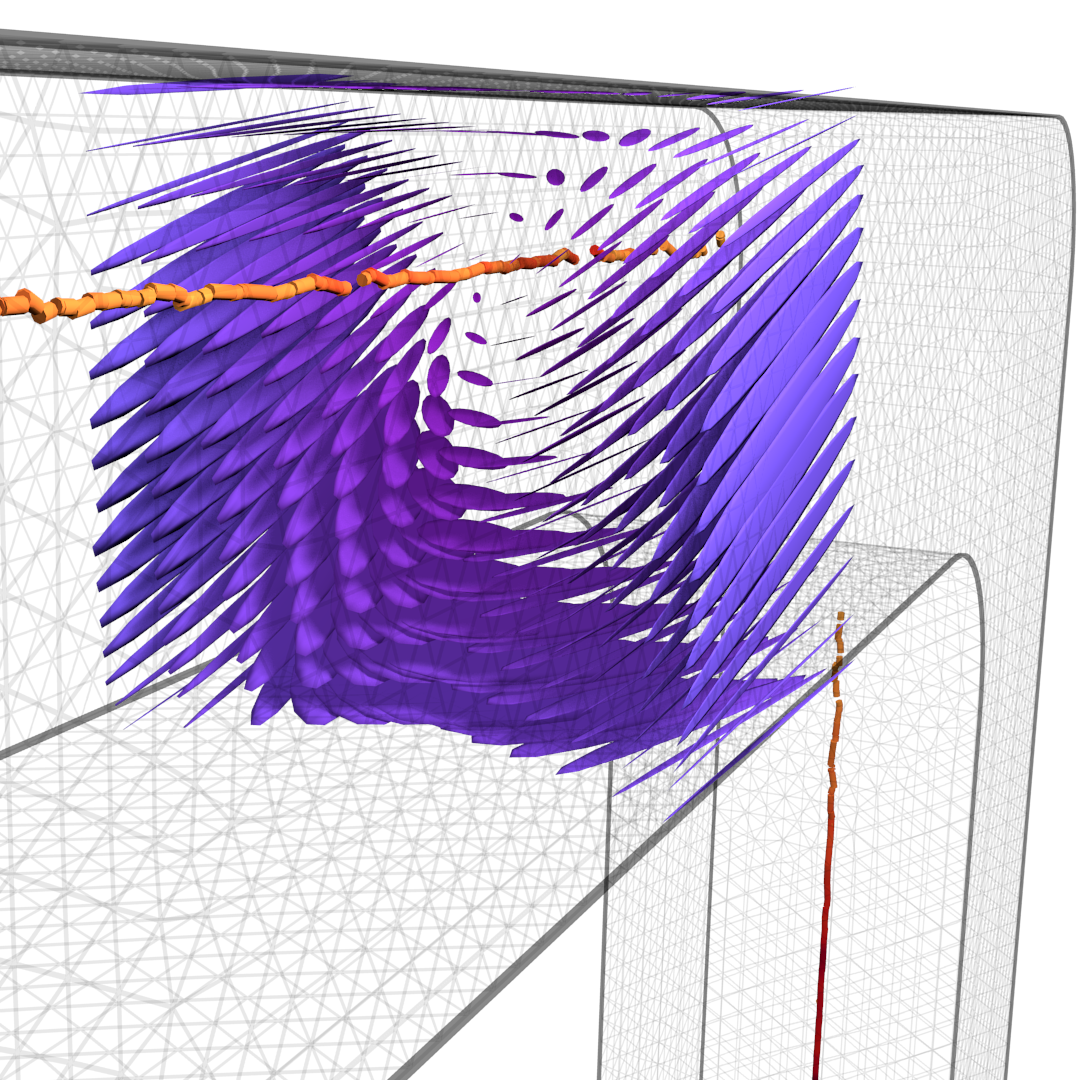
\includegraphics[width=0.305\figurewidth]{figures/hook2_detail2}%
    };

    \node[image, right=of image1] (image5)
    {
        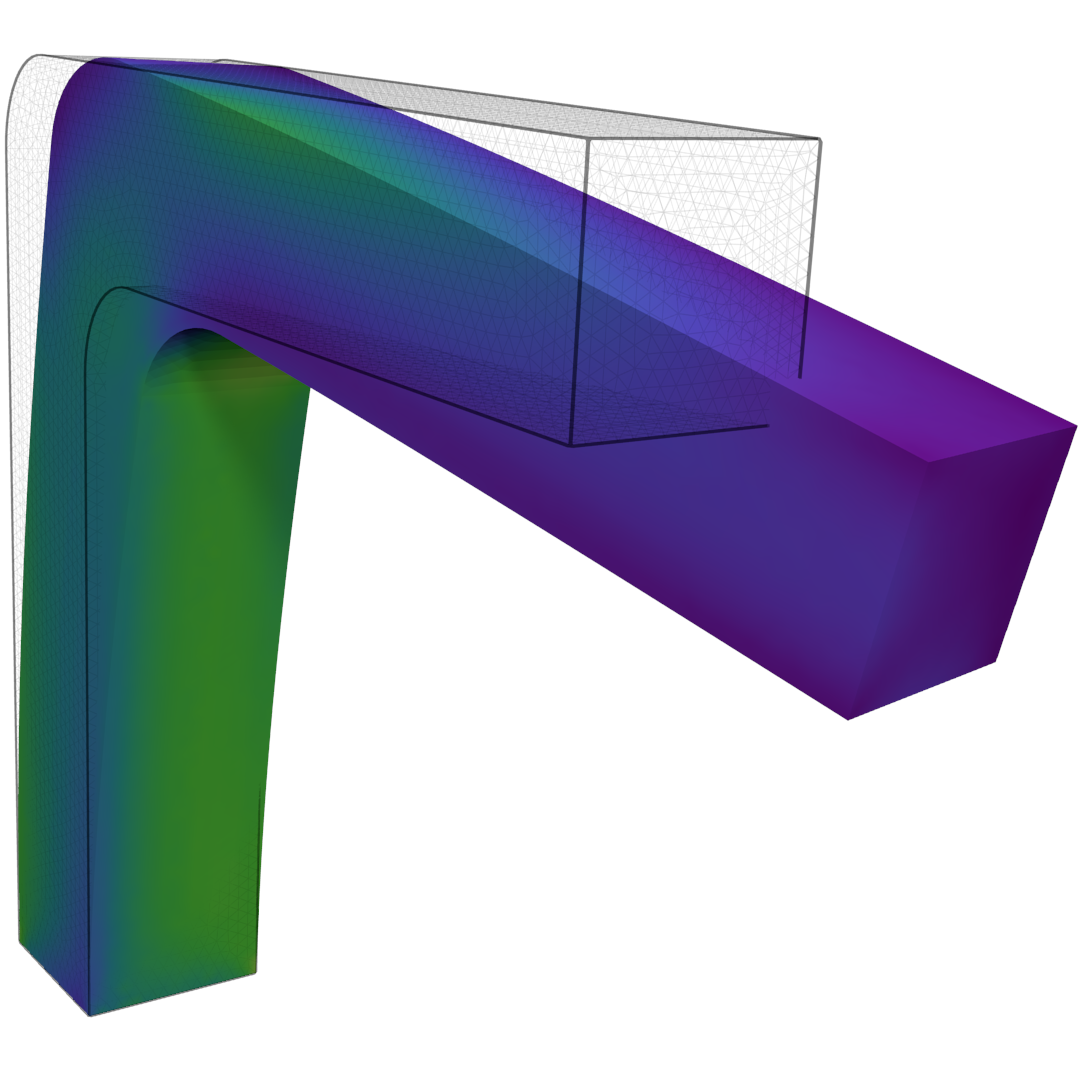
\includegraphics[width=0.305\figurewidth]{figures/hook3_deformation}%
    };

    \node[image, below=of image5] (image6)
    {
        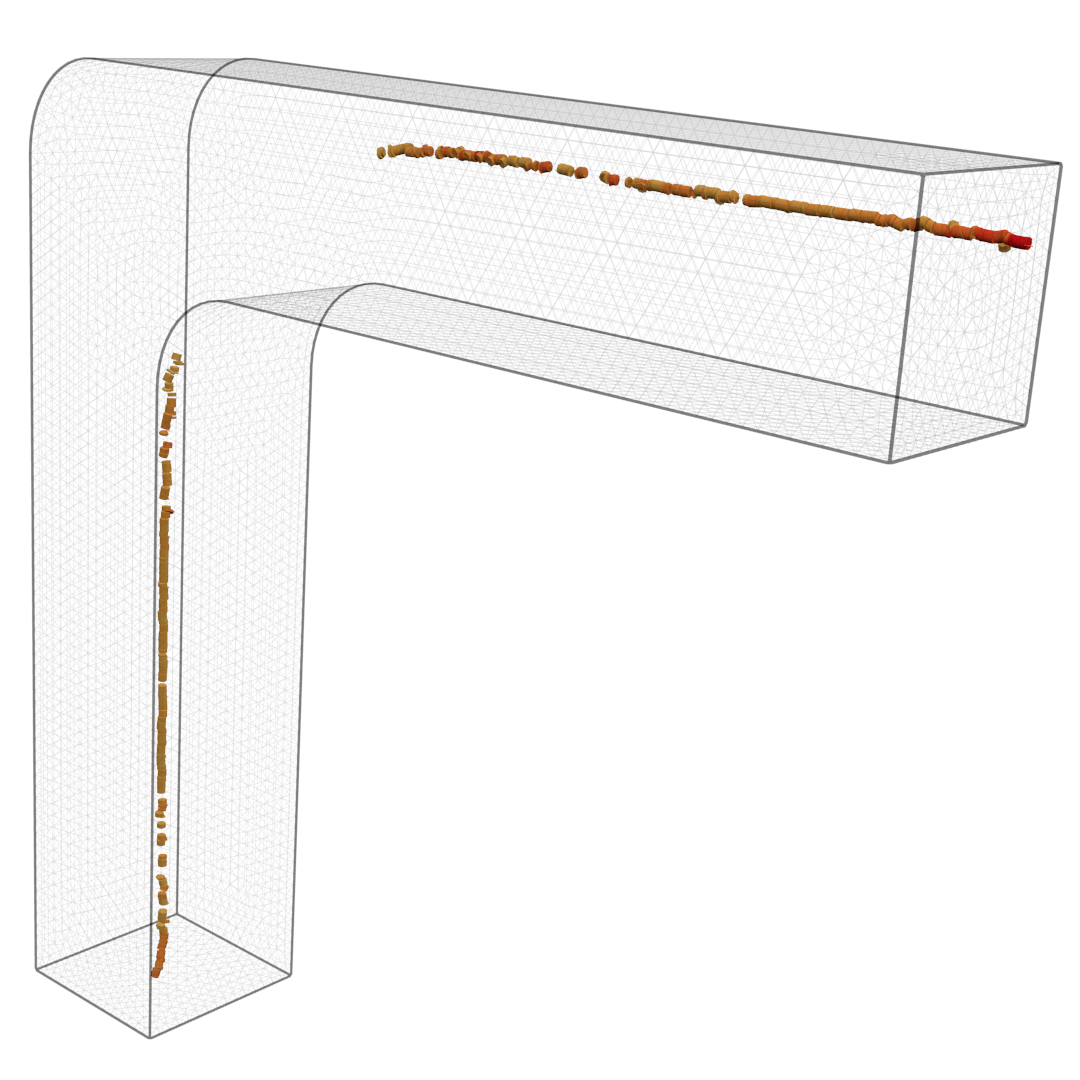
\includegraphics[width=0.305\figurewidth]{figures/hook3_lines}%
    };

    \node[image, below=of image6] (image7)
    {
        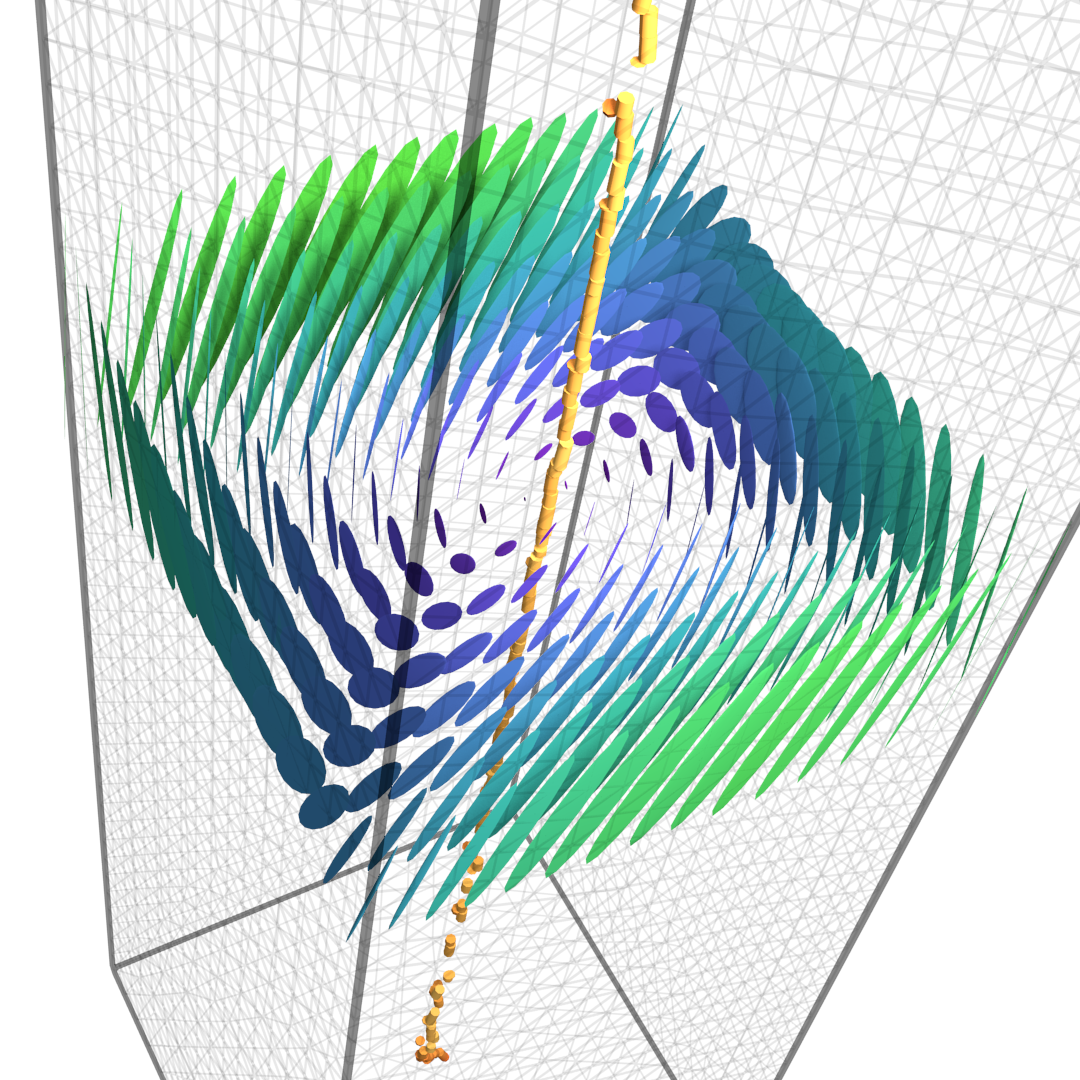
\includegraphics[width=0.305\figurewidth]{figures/hook3_detail1}%
    };

    \node[image, below=of image7] (image8)
    {
        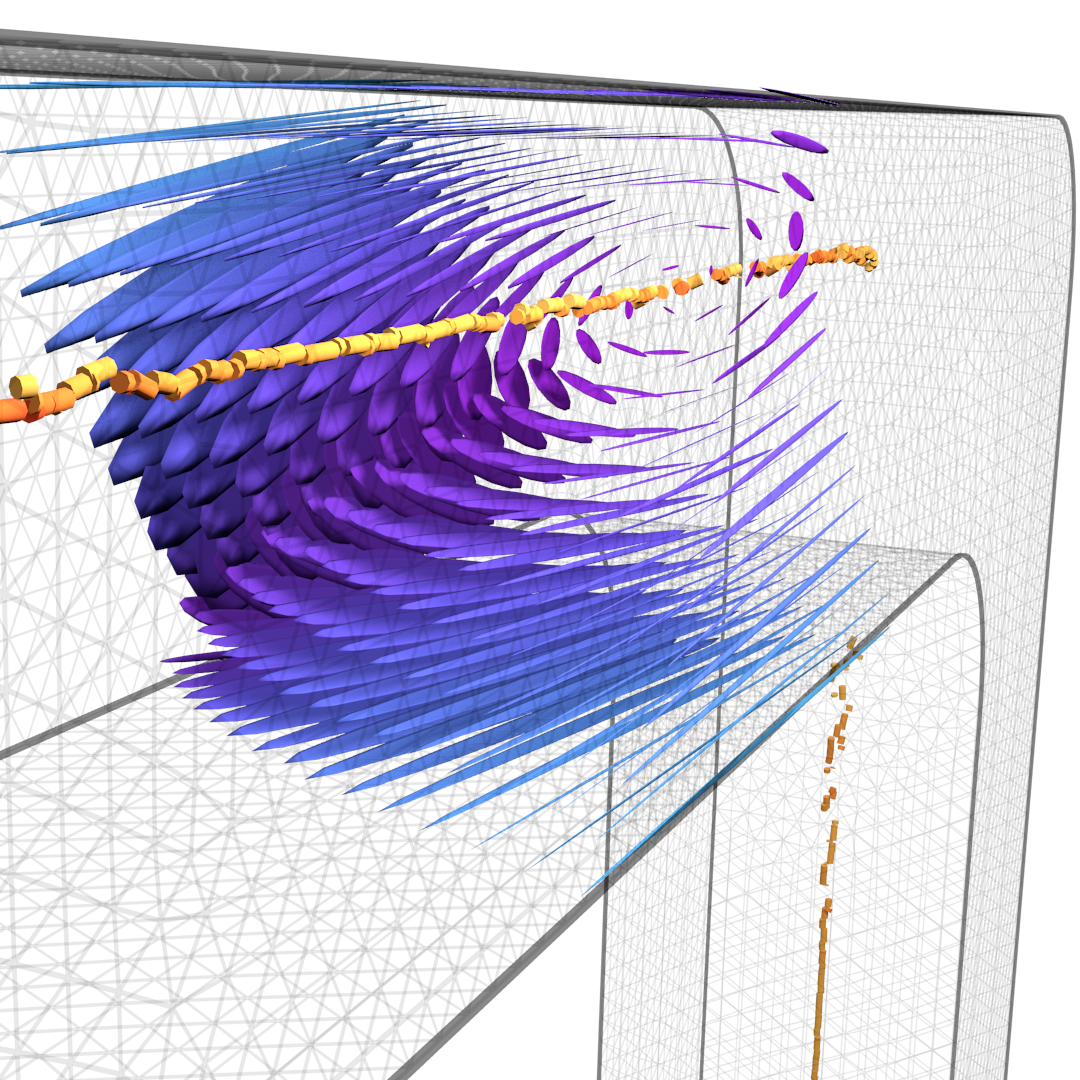
\includegraphics[width=0.305\figurewidth]{figures/hook3_detail2}%
    };

    % This is how you can add a color scale

    \node[anchor=south west, yshift=-4mm] (stabscale) at (image8.south east){
        \begin{axis}[
            scale only axis,
            height=2.8cm,
            hide axis,
            domain=1:20,
            colorbar,
            colorbar/width=0.25cm,
            colormap name={rdoryl},
            point meta min=-5, point meta max=11,
            colorbar style={
                title=$\log(s)$,
                scaled ticks=false,
                ytick={-5, 11}
            }]
        \end{axis}
    };
    \node[anchor=south west, xshift=1.3mm] at (stabscale.north west){
        \begin{axis}[
            scale only axis,
            height=2.8cm,
            hide axis,
            domain=1:20,
            colorbar,
            colorbar/width=0.25cm,
            colormap name={cubicyf},
            point meta min=0, point meta max=8e9,
            colorbar style={
                title=$\sigma_{\text{vM}}$,
                scaled ticks=false,
                ytick={0, 8e9}
            }]
        \end{axis}
    };

\end{tikzpicture}
    \caption{Tensor core lines for two different deformations induced in a
             handle-like object by applying a displacement to an end surface. On
             the left side, we show the resulting deformations. The von Mises
             stress $\sigma_{\text{vM}}$ is color-coded on the surface. We
             represent the tensor core line as tubes in the undeformed
             coordinate system. Their color indicates the numerical stability
             $s$. The tensor field is shown for context using elliptical
             glyphs.}
    \label{fig:hooks}
\end{figure*}
%
This case shows a handle-like structure with a right angle being deformed in
two different ways.
%
One end is fixed, while the other end experiences different displacements.
%
The first is a rotation around the shaft, which applies a torque to it.
%
The second includes an additional downward shift.
%
\autoref{fig:hooks} shows a tensor core line in the center of the shaft for both
cases.
%
Interestingly, a line is also visible in the ``handle''-part of the structure,
even though no direct torque was applied here.
%
The line in the handle shifts away from the plane of symmetry in the second
deformation case.
%
A look at the tensor field around the core lines confirms that they are indeed
the center of a swirling behavior of the tensor field.
%
% subsection hook (end)
%
\paragraph*{Truck Bumper} % (fold)
\label{sub:truck_bumper}
%
This case shows a load applied to the extreme end of the bumper of a cargo
truck.
%
Applying our algorithm to the dataset results in a large number of lines being
found all over the domain.
%
This may in part be explained by the low resolution of the simulation.
%
After applying a filter on the numeric stability $s$, two lines with high
stability stand out.
%
Somewhat counterintuitively, these are found on the side opposite to the end
experiencing the load.
%
In \autoref{fig:truck_bumper}, we can clearly see the radial behavior of the
tensor field around both lines.
%
Finding these locations by manually inspecting the tensor field in detail would
be a tedious task.
%
Using the tensor core line extractor, they can be identified at a glance.
%
\begin{figure*}
    \centering
    \setlength\figurewidth\linewidth
    %
%
\pgfplotsset{colormap={cubicyf}{
rgb = (0.5151, 0.0482, 0.66969999999999996)
rgb = (0.52071100000000003, 0.16895499999999999, 0.80057400000000001)
rgb = (0.49369400000000002, 0.27859600000000001, 0.91182399999999997)
rgb = (0.44002599999999997, 0.369475, 0.98497800000000002)
rgb = (0.39893200000000001, 0.45759300000000003, 0.98705299999999996)
rgb = (0.35065099999999999, 0.54064400000000001, 0.92960799999999999)
rgb = (0.29882700000000001, 0.61562499999999998, 0.85772899999999996)
rgb = (0.239928, 0.68506100000000003, 0.76953099999999997)
rgb = (0.22883200000000001, 0.73934900000000003, 0.67328699999999997)
rgb = (0.263297, 0.78608, 0.56998800000000005)
rgb = (0.29810700000000001, 0.82833699999999999, 0.46021400000000001)
rgb = (0.33091999999999999, 0.86407100000000003, 0.35267399999999999)
rgb = (0.38306000000000001, 0.898169, 0.28730899999999998)
rgb = (0.49023, 0.91748099999999999, 0.30796099999999998)
rgb = (0.62372000000000005, 0.92602600000000002, 0.33230900000000002)
rgb = (0.71745800000000004, 0.92527000000000004, 0.342476)
rgb = (0.80000000000000004, 0.92549999999999999, 0.35289999999999999)
}}
\pgfplotsset{colormap={rdoryl}{
rgb(0)=(1, 1, 0.80000000000000004)
rgb(1)=(1, 0.96678200000000003, 0.71879999999999999)
rgb(2)=(1, 0.93134899999999998, 0.63218799999999997)
rgb(3)=(0.998139, 0.89219499999999996, 0.54929600000000001)
rgb(4)=(0.99617100000000003, 0.85282599999999997, 0.46662100000000001)
rgb(5)=(0.99607800000000002, 0.77780899999999997, 0.38394499999999998)
rgb(6)=(0.99607800000000002, 0.70103800000000005, 0.30126900000000001)
rgb(7)=(0.99418700000000004, 0.62805100000000003, 0.26777400000000001)
rgb(8)=(0.99221800000000004, 0.55521699999999996, 0.23627799999999999)
rgb(9)=(0.99024999999999996, 0.43280299999999999, 0.20096900000000001)
rgb(10)=(0.98828099999999997, 0.30878899999999998, 0.16553599999999999)
rgb(11)=(0.94017700000000004, 0.20592099999999999, 0.137793)
rgb(12)=(0.89096500000000001, 0.10356, 0.110235)
rgb(13)=(0.81656300000000004, 0.051580000000000001, 0.12918099999999999)
rgb(14)=(0.741761, 0.00040000000000000002, 0.148866)
rgb(15)=(0.62203799999999998, 0, 0.14902000000000001)
rgb(16)=(0.50196099999999999, 0, 0.14902000000000001)
}}
%
\begin{tikzpicture}
    \tikzstyle{image} = [inner sep=0, outer sep=0, node distance = 0 and 0]

    % place image in node
    \node[image] (image1)
    {
        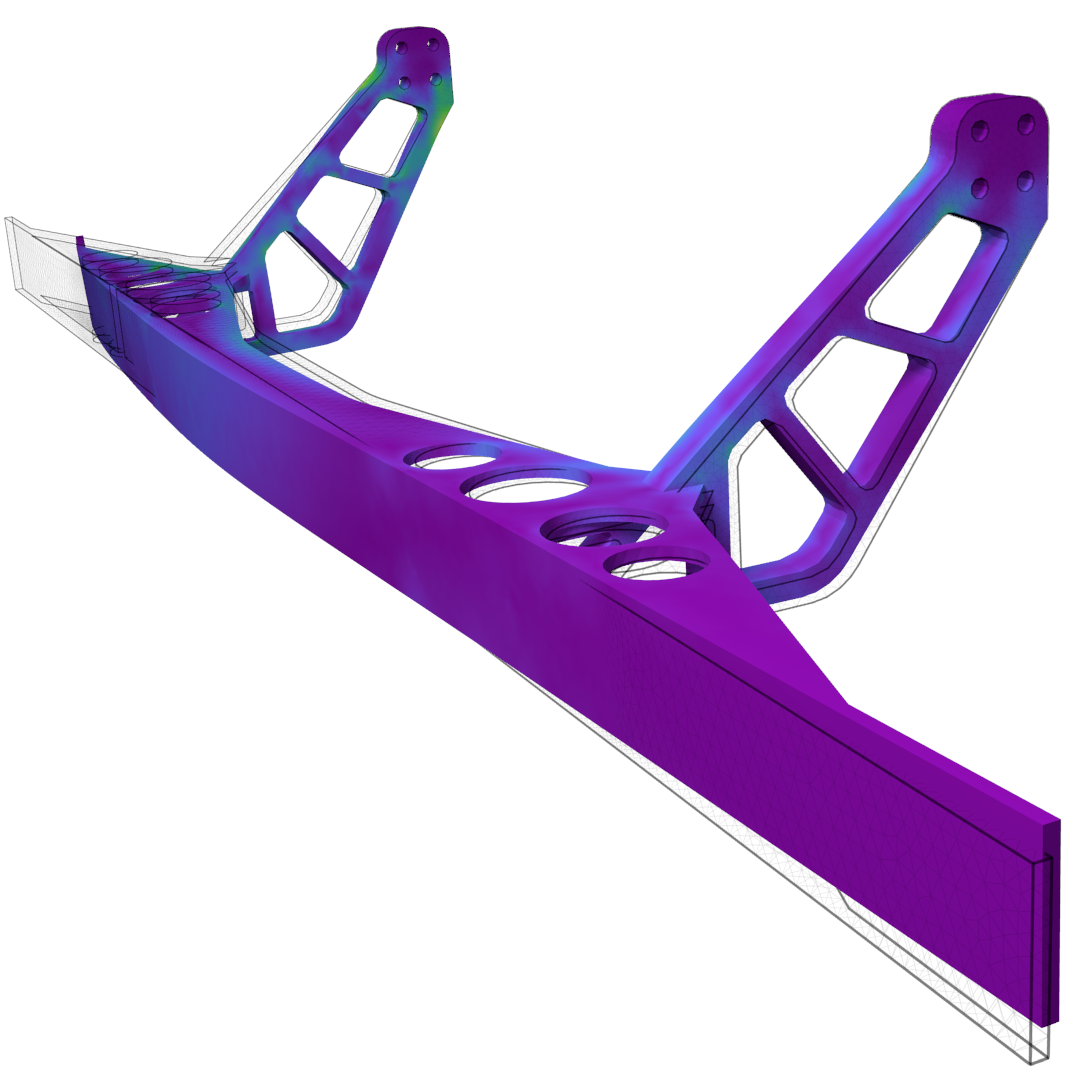
\includegraphics[width=0.22\figurewidth]{figures/truck_bumper_deformation}%
    };

    % place next image to the right with a little space in between
    \node[image, right=of image1, xshift=0.25cm] (image2)
    {
        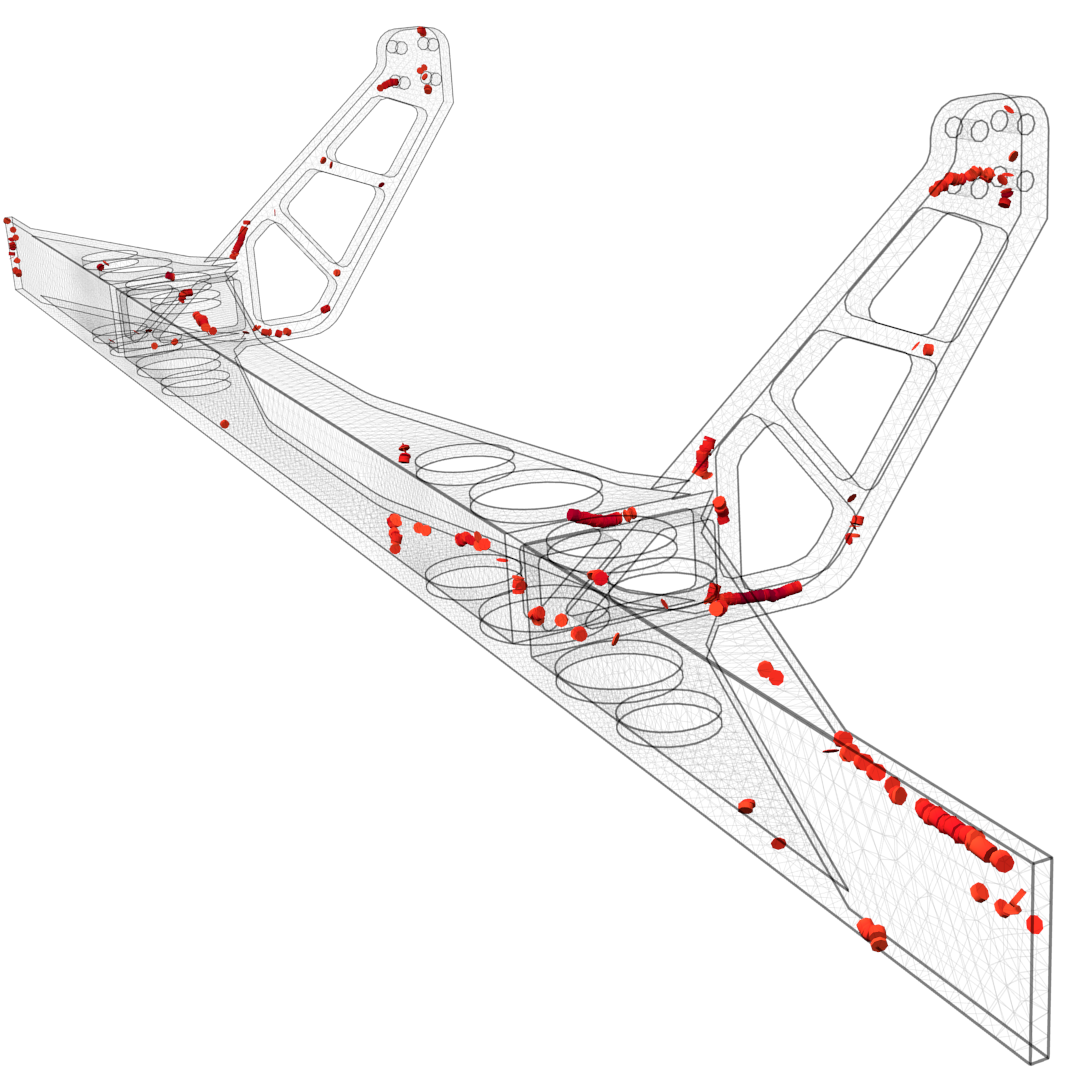
\includegraphics[width=0.22\figurewidth]{figures/truck_bumper_lines}%
    };
    % create new coordinate system on image2:
    \begin{scope}[
        shift=(image2.south west), % origin is lower left corner
        x={($(image2.south east)-(image2.south west)$)}, % x axis is lower side
        y={($(image2.north west)-(image2.south west)$)}] % y axis is left side
        % uncomment the following three lines to show a helper grid that helps
        % with finding coordinates
        % \draw[help lines,xstep=.1,ystep=.1] (0,0) grid (1,1);
        % \foreach \x in {0,1,...,9} { \node [anchor=north] at (\x/10,0) {\scriptsize 0.\x}; }
        % \foreach \y in {0,1,...,9} { \node [anchor=east] at (0,\y/10) {\scriptsize 0.\y}; }
        % draw stuff on image
        % (0, 0) is lower left corner, (1, 1) is upper right
        \draw [thin, -] (0.55, 0.535) -- (0.55, 0.6) node [anchor=south] {\large \textbf{$1$}};
        \draw [thin, -] (0.72, 0.435) -- (0.8, 0.4) node [anchor=west] {\large \textbf{$2$}};
    \end{scope}

    \node[image, right=of image2, xshift=0.25cm] (image3)
    {
        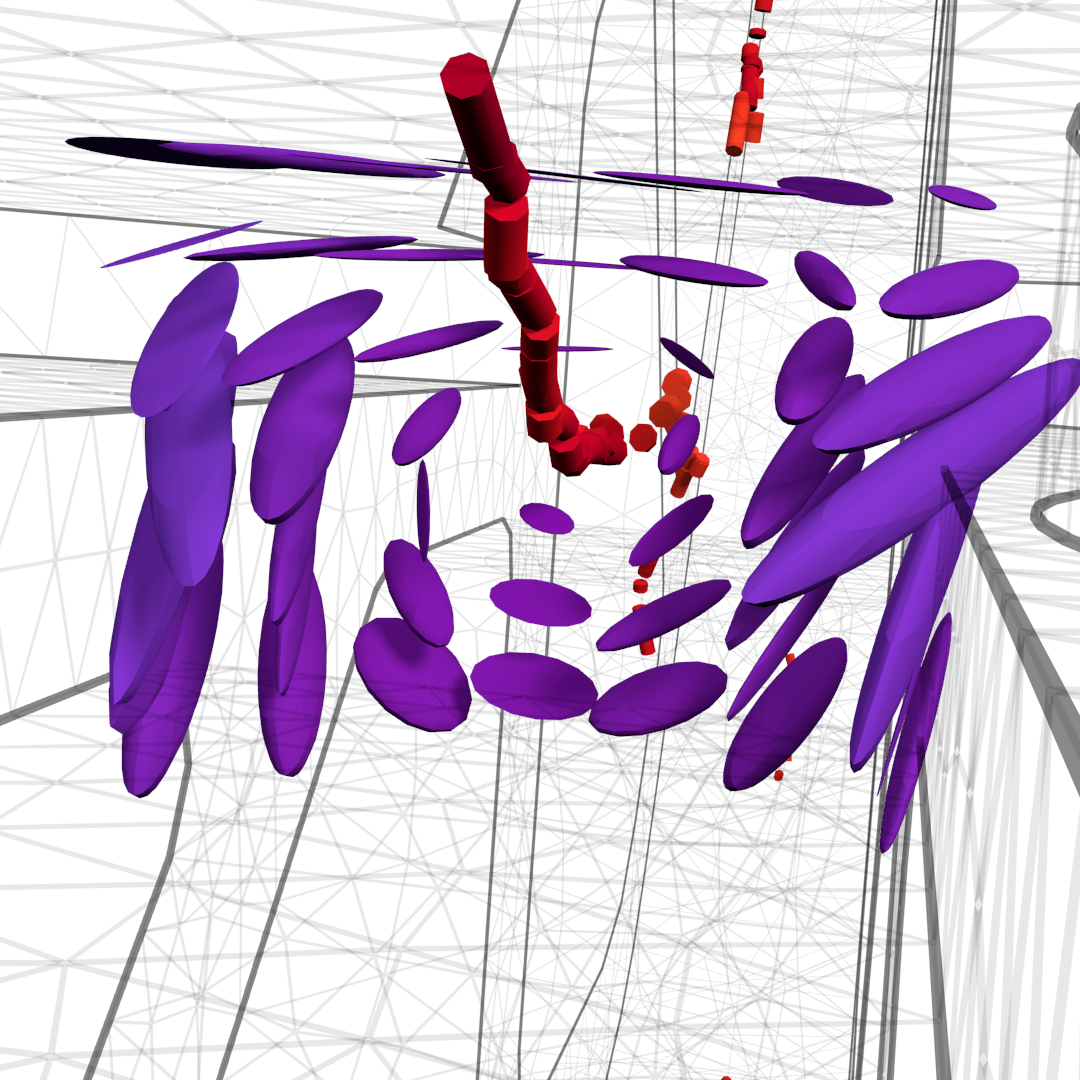
\includegraphics[width=0.22\figurewidth]{figures/truck_bumper_detail2}%
    };
    % place a text on the lower left corner of image3
    \node [anchor=south west] at (image3.south west) {\LARGE \textbf{$1$}};

    \node[image, right=of image3, xshift=0.25cm] (image4)
    {
        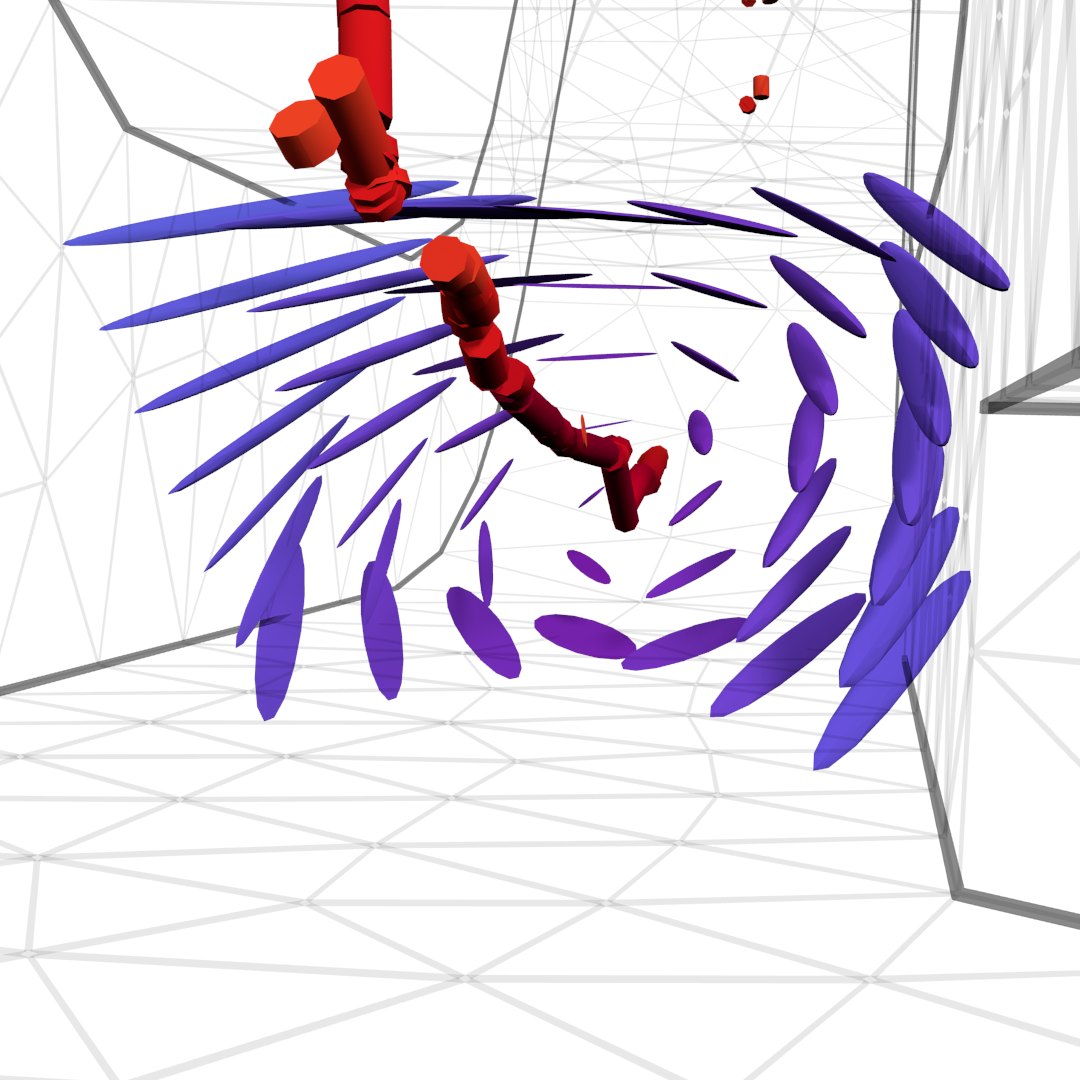
\includegraphics[width=0.22\figurewidth]{figures/truck_bumper_detail1}%
    };
    \node [anchor=south west] at (image4.south west) {\LARGE \textbf{$2$}};

    \node[anchor=north west, xshift=-0.7cm, yshift=0.15cm] at (image4.north east){
        \begin{axis}[
            scale only axis,
            height=1.1cm,
            hide axis,
            domain=1:20,
            colorbar,
            colorbar/width=0.25cm,
            colormap name={cubicyf},
            point meta min=0, point meta max=9e6,
            colorbar style={
                title=$\sigma_{\text{vM}}$,
                scaled ticks=false,
                ytick={0, 9e6}
            }]
        \end{axis}
    };
    \node[anchor=south west, xshift=-0.8cm, yshift=-0.15cm] at (image4.south east){
        \begin{axis}[
            scale only axis,
            height=1.1cm,
            hide axis,
            domain=1:20,
            colorbar,
            colorbar/width=0.25cm,
            colormap name={rdoryl},
            point meta min=1.5, point meta max=15,
            colorbar style={
                title=$\log(s)$,
                scaled ticks=false,
                ytick={1.5, 15}
            }]
        \end{axis}
    };

\end{tikzpicture}
    \caption{Tensor core lines in a truck bumper with a load applied to one end.
             The deformation shown on the left is scaled 500 times for
             illustrative purposes. The right shows detail views of two
             interesting lines.}
    \label{fig:truck_bumper}
\end{figure*}
%
% subsection truck_bumper (end)
%
\paragraph*{Crane} % (fold)
\label{sub:crane}
%
In this dataset, the arm of a crane is exposed to a downward pull applied to
the lower side of a cube at the end (see \autoref{fig:crane}).
%
Similar to the truck bumper, it is not intuitively clear in which parts of the
structure a swirling behavior of the tensors will occur, just from looking at
the setup of the case.
%
Almost all stable solutions we find are located in the diagonal rods on the
lower side.
%
Again, looking closely at the tensors around the core lines, we can see the
radial behavior.
%
\begin{figure*}
    \centering
    \setlength\figurewidth\linewidth
    %
%
\pgfplotsset{colormap={cubicyf}{
rgb = (0.5151, 0.0482, 0.66969999999999996)
rgb = (0.52071100000000003, 0.16895499999999999, 0.80057400000000001)
rgb = (0.49369400000000002, 0.27859600000000001, 0.91182399999999997)
rgb = (0.44002599999999997, 0.369475, 0.98497800000000002)
rgb = (0.39893200000000001, 0.45759300000000003, 0.98705299999999996)
rgb = (0.35065099999999999, 0.54064400000000001, 0.92960799999999999)
rgb = (0.29882700000000001, 0.61562499999999998, 0.85772899999999996)
rgb = (0.239928, 0.68506100000000003, 0.76953099999999997)
rgb = (0.22883200000000001, 0.73934900000000003, 0.67328699999999997)
rgb = (0.263297, 0.78608, 0.56998800000000005)
rgb = (0.29810700000000001, 0.82833699999999999, 0.46021400000000001)
rgb = (0.33091999999999999, 0.86407100000000003, 0.35267399999999999)
rgb = (0.38306000000000001, 0.898169, 0.28730899999999998)
rgb = (0.49023, 0.91748099999999999, 0.30796099999999998)
rgb = (0.62372000000000005, 0.92602600000000002, 0.33230900000000002)
rgb = (0.71745800000000004, 0.92527000000000004, 0.342476)
rgb = (0.80000000000000004, 0.92549999999999999, 0.35289999999999999)
}}
\pgfplotsset{colormap={rdoryl}{
rgb(0)=(1, 1, 0.80000000000000004)
rgb(1)=(1, 0.96678200000000003, 0.71879999999999999)
rgb(2)=(1, 0.93134899999999998, 0.63218799999999997)
rgb(3)=(0.998139, 0.89219499999999996, 0.54929600000000001)
rgb(4)=(0.99617100000000003, 0.85282599999999997, 0.46662100000000001)
rgb(5)=(0.99607800000000002, 0.77780899999999997, 0.38394499999999998)
rgb(6)=(0.99607800000000002, 0.70103800000000005, 0.30126900000000001)
rgb(7)=(0.99418700000000004, 0.62805100000000003, 0.26777400000000001)
rgb(8)=(0.99221800000000004, 0.55521699999999996, 0.23627799999999999)
rgb(9)=(0.99024999999999996, 0.43280299999999999, 0.20096900000000001)
rgb(10)=(0.98828099999999997, 0.30878899999999998, 0.16553599999999999)
rgb(11)=(0.94017700000000004, 0.20592099999999999, 0.137793)
rgb(12)=(0.89096500000000001, 0.10356, 0.110235)
rgb(13)=(0.81656300000000004, 0.051580000000000001, 0.12918099999999999)
rgb(14)=(0.741761, 0.00040000000000000002, 0.148866)
rgb(15)=(0.62203799999999998, 0, 0.14902000000000001)
rgb(16)=(0.50196099999999999, 0, 0.14902000000000001)
}}
%
\begin{tikzpicture}[
    font=\small
]
    \tikzstyle{image} = [inner sep=0, outer sep=0, node distance = 0 and 0]

    % place image in node
    \node[image] (image1)
    {
        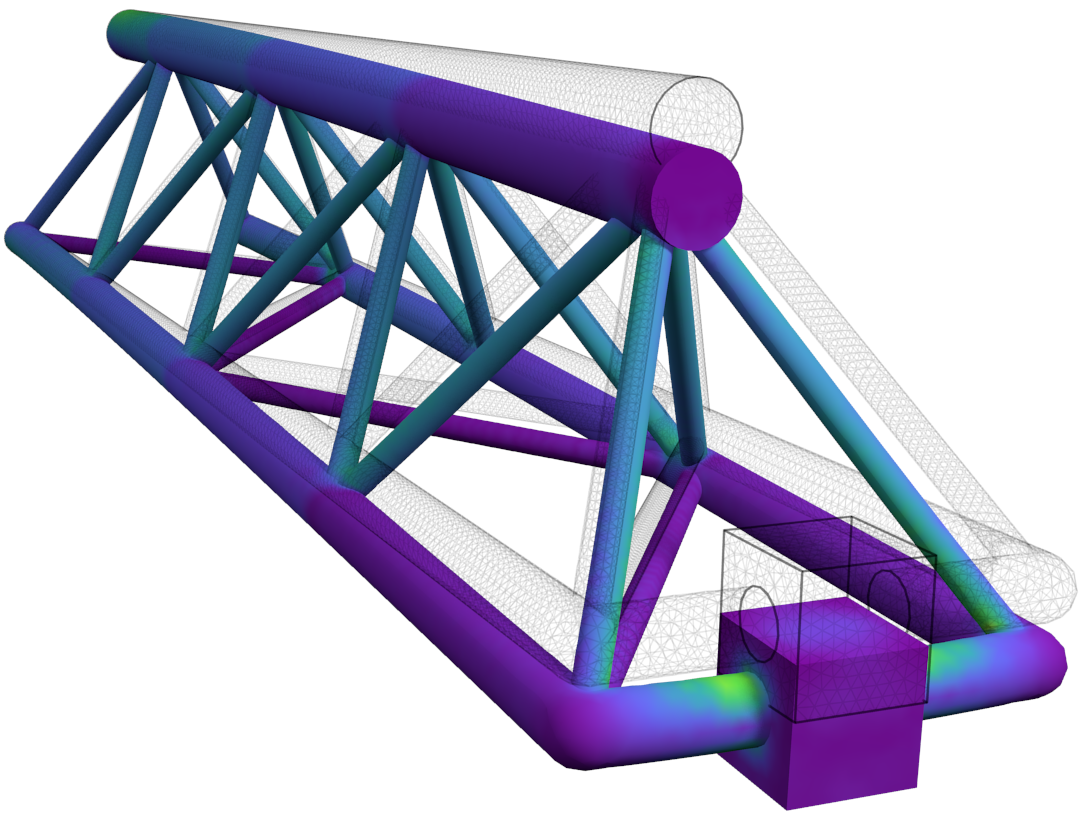
\includegraphics[width=0.333\figurewidth]{figures/crane_deformation}%
    };

    % place next image to the right with a little space in between
    \node[image, right=of image1] (image2)
    {
        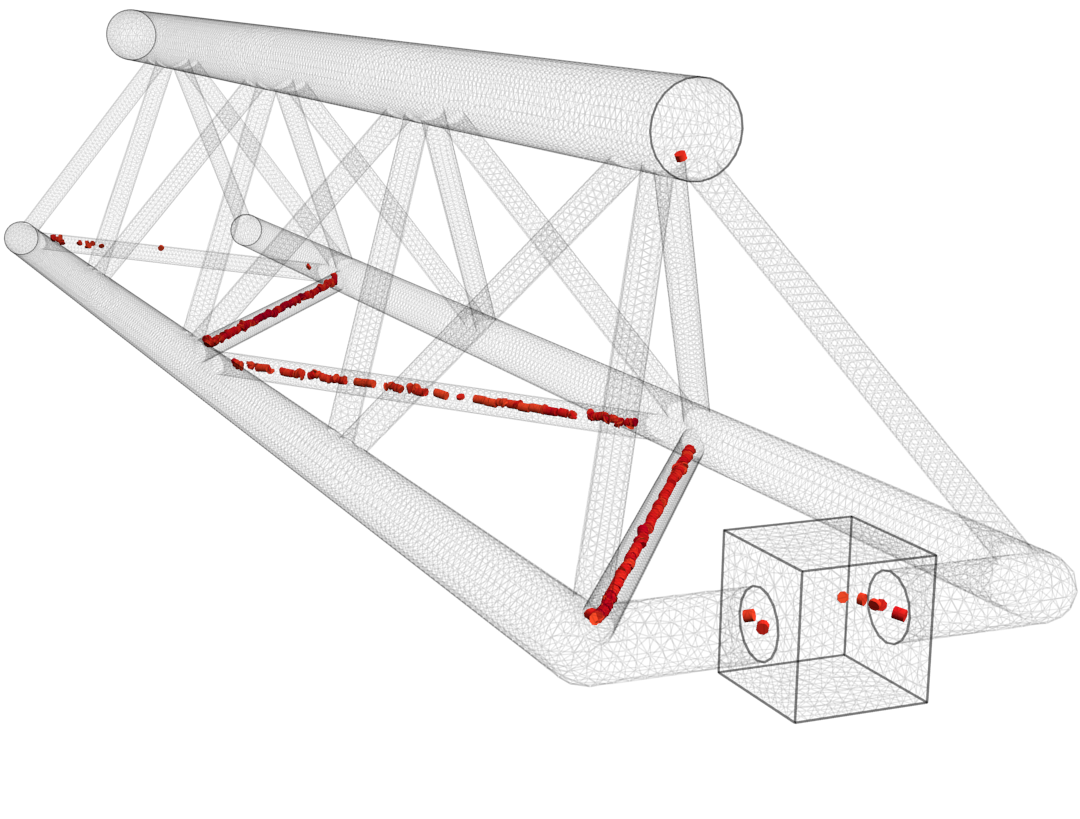
\includegraphics[width=0.333\figurewidth]{figures/crane_lines}%
    };

    \node[image, right=of image2] (image3)
    {
        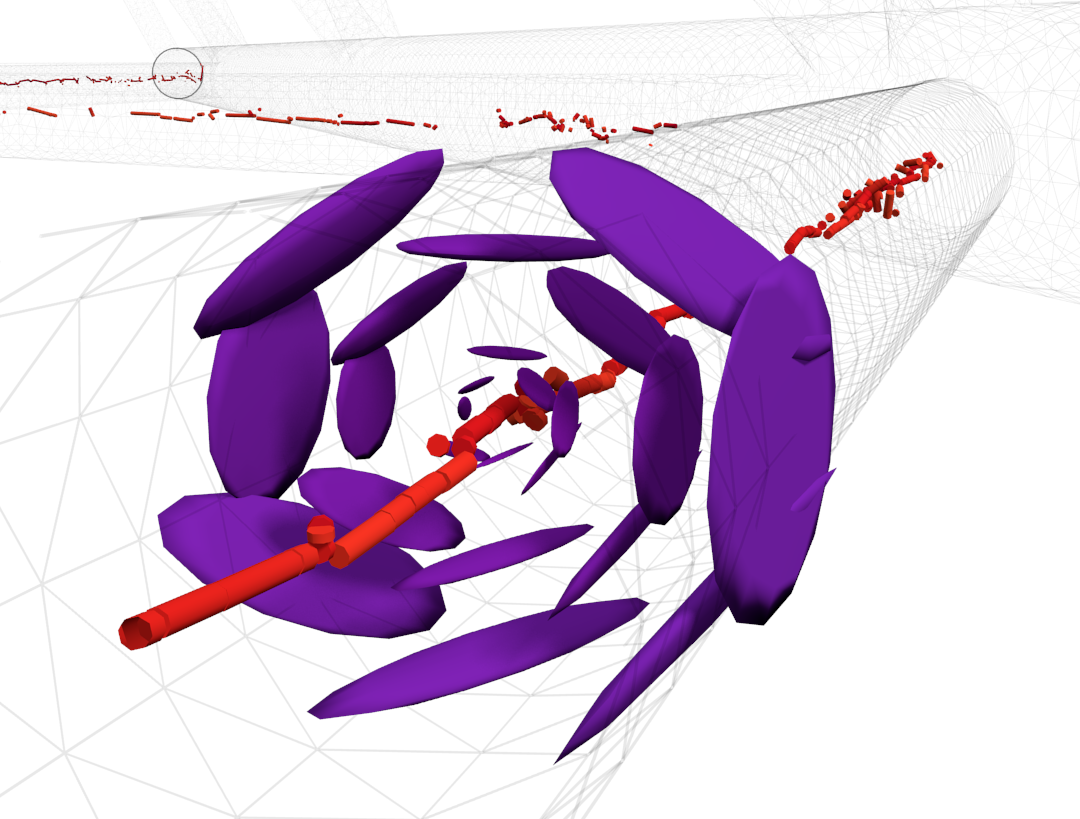
\includegraphics[width=0.333\figurewidth]{figures/crane_detail}%
    };

    \node[anchor=north east] at (image2.south){
        \begin{axis}[
            scale only axis,
            height=2.8cm,
            hide axis,
            domain=1:20,
            colorbar horizontal,
            colorbar/width=0.25cm,
            colormap name={cubicyf},
            point meta min=0, point meta max=1.5e6,
            colorbar style={
                title=\strut$\sigma_{\textnormal{vM}}$,
                scaled ticks=false,
                xtick={0, 1.5e6}
            }]
        \end{axis}
    };
    \node[anchor=north west] at (image2.south){
        \begin{axis}[
            scale only axis,
            height=2.8cm,
            hide axis,
            domain=1:20,
            colorbar horizontal,
            colorbar/width=0.25cm,
            colormap name={rdoryl},
            point meta min=-7.5, point meta max=11,
            colorbar style={
                title=\strut$\log(s)$,
                scaled ticks=false,
                xtick={-7.5, 11}
            }]
        \end{axis}
    };

\end{tikzpicture}
    \caption{Tensor core lines in a crane arm with a load applied to the end.
             The resulting deformation on the left is scaled 1500 times.
             Significant tensor core lines are only found in the lower diagonal
             rods. The detail image on the right shows the tensors are indeed
             aligned around a common core.}
    \label{fig:crane}
\end{figure*}
%
% subsection crane (end)
%
\paragraph*{Spring} % (fold)
\label{sub:spring}
%
A simulation of a coil spring being compressed and slightly bent between two
plates is shown in~\autoref{fig:spring}.
%
Apart from numerical noise in the poorly resolved plates, we find significant
tensor core lines at the center of the coil's cross-section.
%
A look at the tensor field visualized by glyphs reveals that in this case, we
do not have a simple swirling behavior of the tensors.
%
Instead, the tensor field shows something similar to a hyperbolic behavior in
vector fields.
%
In the rightmost picture in~\autoref{fig:spring}, we can see that eigenvector
trajectories start at the wall on both sides and curve into the same direction.
%
This direction is reversed on the top and bottom side of the spring.
%
In the middle, there is a surface where these curves become straight lines along
the diameter of the cross-section.
%
This is exactly where we find a tensor core line.
%
\begin{figure*}
    \centering
    \setlength\figurewidth\linewidth
    %
%
\pgfplotsset{colormap={cubicyf}{
rgb = (0.5151, 0.0482, 0.66969999999999996)
rgb = (0.52071100000000003, 0.16895499999999999, 0.80057400000000001)
rgb = (0.49369400000000002, 0.27859600000000001, 0.91182399999999997)
rgb = (0.44002599999999997, 0.369475, 0.98497800000000002)
rgb = (0.39893200000000001, 0.45759300000000003, 0.98705299999999996)
rgb = (0.35065099999999999, 0.54064400000000001, 0.92960799999999999)
rgb = (0.29882700000000001, 0.61562499999999998, 0.85772899999999996)
rgb = (0.239928, 0.68506100000000003, 0.76953099999999997)
rgb = (0.22883200000000001, 0.73934900000000003, 0.67328699999999997)
rgb = (0.263297, 0.78608, 0.56998800000000005)
rgb = (0.29810700000000001, 0.82833699999999999, 0.46021400000000001)
rgb = (0.33091999999999999, 0.86407100000000003, 0.35267399999999999)
rgb = (0.38306000000000001, 0.898169, 0.28730899999999998)
rgb = (0.49023, 0.91748099999999999, 0.30796099999999998)
rgb = (0.62372000000000005, 0.92602600000000002, 0.33230900000000002)
rgb = (0.71745800000000004, 0.92527000000000004, 0.342476)
rgb = (0.80000000000000004, 0.92549999999999999, 0.35289999999999999)
}}
\pgfplotsset{colormap={rdoryl}{
rgb(0)=(1, 1, 0.80000000000000004)
rgb(1)=(1, 0.96678200000000003, 0.71879999999999999)
rgb(2)=(1, 0.93134899999999998, 0.63218799999999997)
rgb(3)=(0.998139, 0.89219499999999996, 0.54929600000000001)
rgb(4)=(0.99617100000000003, 0.85282599999999997, 0.46662100000000001)
rgb(5)=(0.99607800000000002, 0.77780899999999997, 0.38394499999999998)
rgb(6)=(0.99607800000000002, 0.70103800000000005, 0.30126900000000001)
rgb(7)=(0.99418700000000004, 0.62805100000000003, 0.26777400000000001)
rgb(8)=(0.99221800000000004, 0.55521699999999996, 0.23627799999999999)
rgb(9)=(0.99024999999999996, 0.43280299999999999, 0.20096900000000001)
rgb(10)=(0.98828099999999997, 0.30878899999999998, 0.16553599999999999)
rgb(11)=(0.94017700000000004, 0.20592099999999999, 0.137793)
rgb(12)=(0.89096500000000001, 0.10356, 0.110235)
rgb(13)=(0.81656300000000004, 0.051580000000000001, 0.12918099999999999)
rgb(14)=(0.741761, 0.00040000000000000002, 0.148866)
rgb(15)=(0.62203799999999998, 0, 0.14902000000000001)
rgb(16)=(0.50196099999999999, 0, 0.14902000000000001)
}}
%
\begin{tikzpicture}[
    font=\small
]
    \tikzstyle{image} = [inner sep=0, outer sep=0, node distance = 0 and 0]

    \node[image] (image1)
    {
        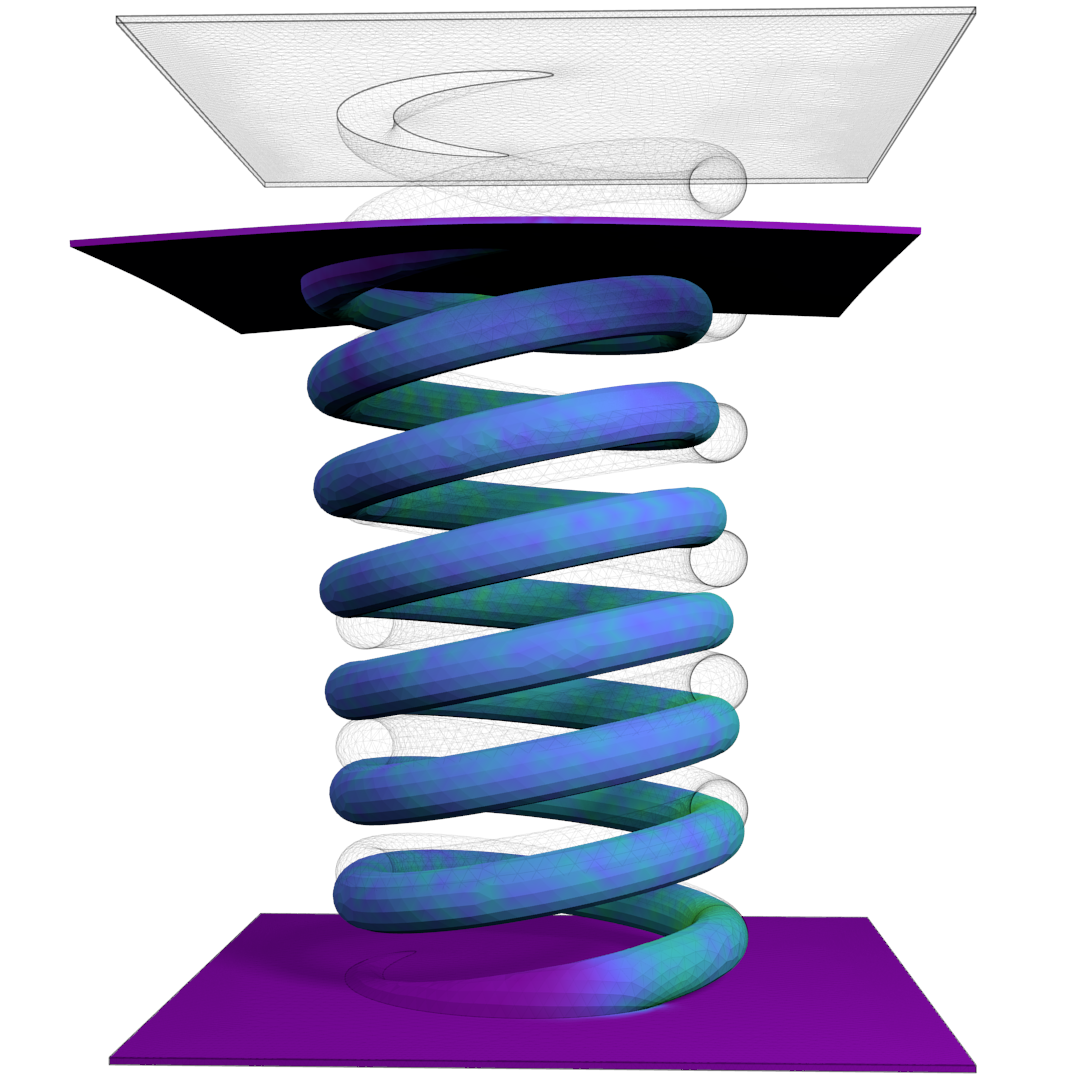
\includegraphics[width=0.22\figurewidth]{figures/spring_deformation}%
    };

    \node[image, right=of image1, xshift=0.25cm] (image2)
    {
        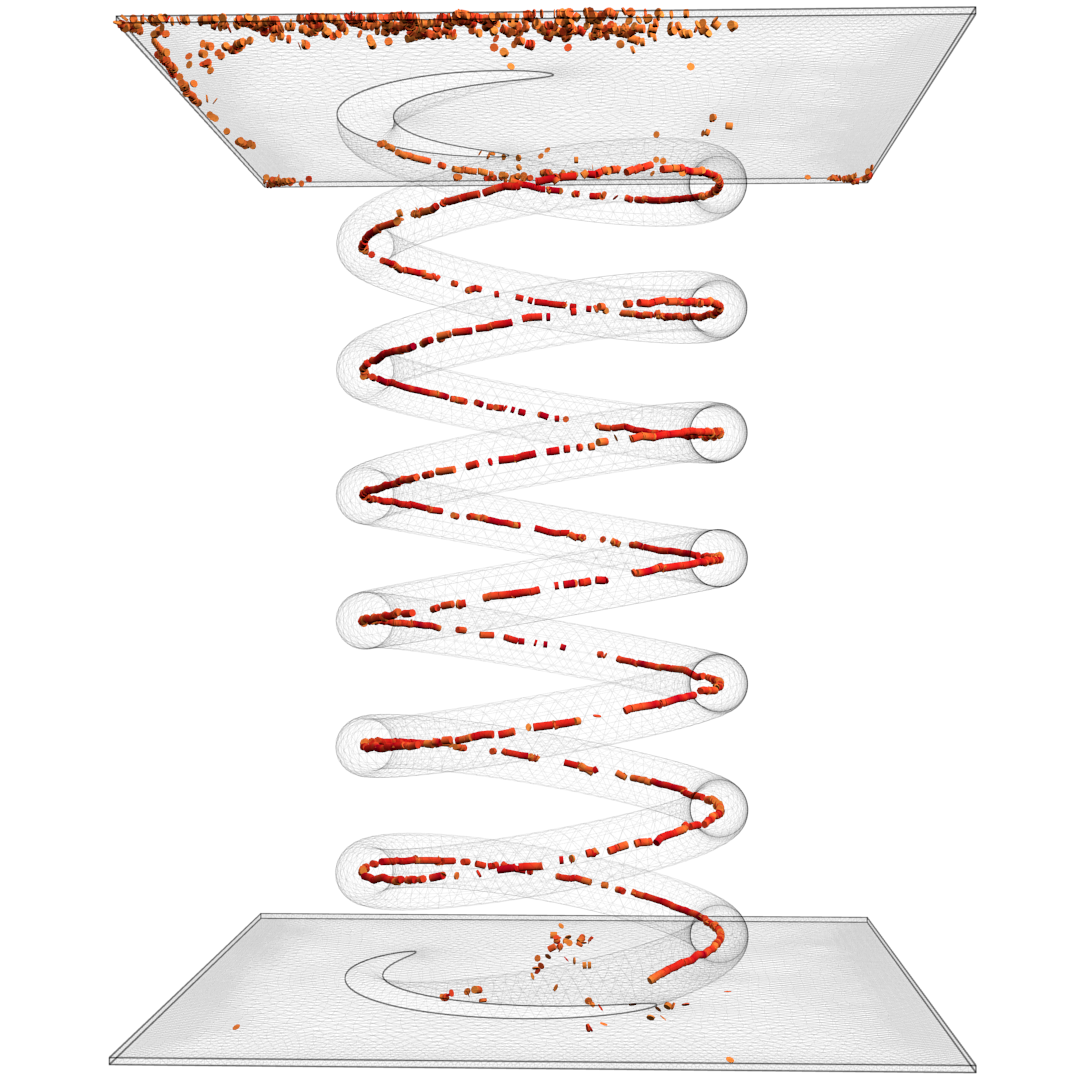
\includegraphics[width=0.22\figurewidth]{figures/spring_lines}%
    };

    \node[image, right=of image2, xshift=0.25cm] (image3)
    {
        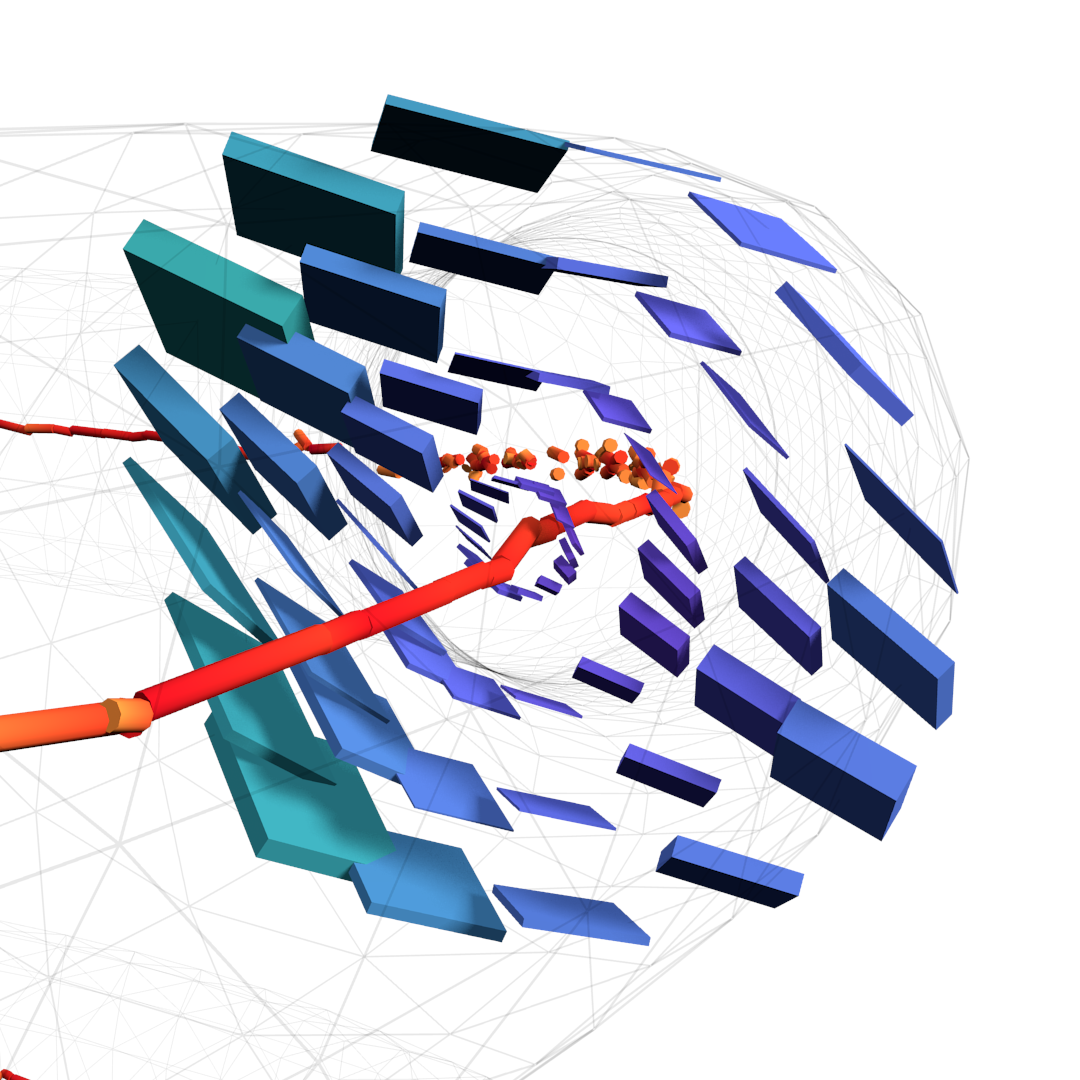
\includegraphics[width=0.22\figurewidth]{figures/spring_detail1_box}%
    };

    \node[image, right=of image3, xshift=0.25cm] (image4)
    {
        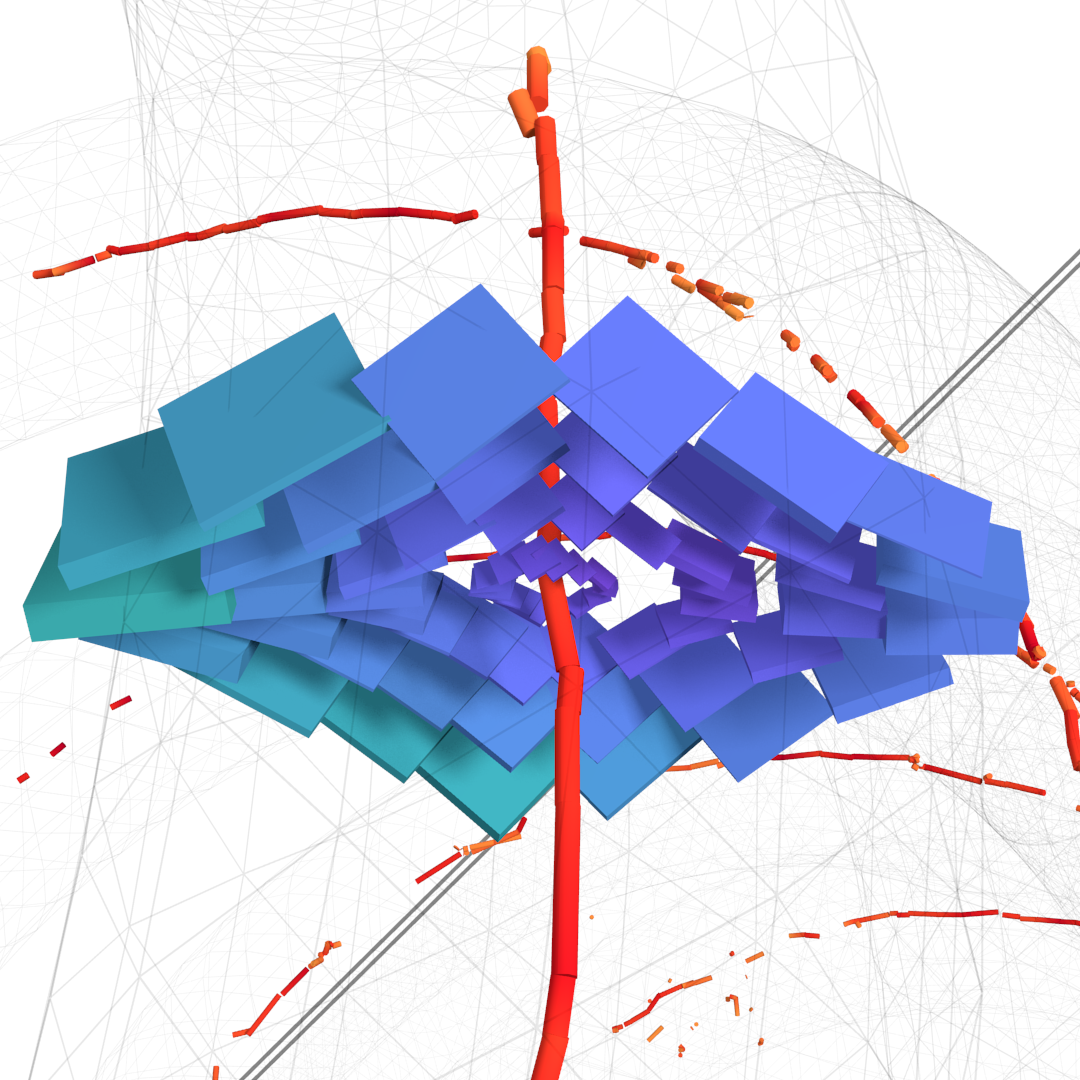
\includegraphics[width=0.22\figurewidth]{figures/spring_detail2_box}%
    };

    \node[anchor=north west, xshift=-0.7cm, yshift=0.15cm] at (image4.north east){
        \begin{axis}[
            scale only axis,
            height=1.1cm,
            hide axis,
            domain=1:20,
            colorbar,
            colorbar/width=0.25cm,
            colormap name={cubicyf},
            point meta min=0, point meta max=1e9,
            colorbar style={
                title=$\sigma_{\text{vM}}$,
                scaled ticks=false,
                ytick={0, 1e9}
            }]
        \end{axis}
    };
    \node[anchor=south west, xshift=-0.8cm, yshift=-0.15cm] at (image4.south east){
        \begin{axis}[
            scale only axis,
            height=1.1cm,
            hide axis,
            domain=1:20,
            colorbar,
            colorbar/width=0.25cm,
            colormap name={rdoryl},
            point meta min=3, point meta max=17,
            colorbar style={
                title=$\log(s)$,
                scaled ticks=false,
                ytick={3, 17}
            }]
        \end{axis}
    };

\end{tikzpicture}
    \caption{A coil spring being compressed and slightly bent between two
             plates. We visualize the tensors near the core line with box glyphs
             in this case. They make it easier to see the hyperbolic behavior of
             the eigenvectors that occurs in the coil's cross-section. }
    \label{fig:spring}
\end{figure*}
%
% subsection spring (end)
%
\subsection{Performance and Parameter Study} % (fold)
\label{sub:performance}
%
The performance of our algorithm is dependent on the dataset.
%
If we find a large number of tensor core lines in the dataset, computation
will be slower as fewer cells can be discarded early.
%
We tested our algorithm using a consumer PC with a 4-core Intel Core i7 CPU at
\SI{3.4}{\giga\hertz}.
%
Our implementation is parallelized over the faces of the dataset using
OpenMP~\cite{OMP2013}.
%
Performance numbers for the different datasets shown in this paper are presented
in \autoref{tab:performance}.
%
To examine the dependence of the performance and results of our algorithm on the
parameters $M$, $\varepsilon_{\mathrm{t}}$ and $\varepsilon_{\mathrm{c}}$, we
conducted a parameter study.
%
We selected baseline parameters $M = 10^3$, $\varepsilon_{\mathrm{t}} =
\num{1e-6}$ and $\varepsilon_{\mathrm{c}} = \num{1e-3}$.
%
We then varied each parameter separately and applied our algorithm to the
cylinder dataset.
%
The results can be seen in \autoref{fig:parameter_study}.
%
We can see that the performance is controlled by the threshold $M$, which
controls at which point we assume we are not converging onto an isolated
solution.
%
Increasing $M$ also increases the number of solutions we find.
%
However, if we look at the number of solutions that remain after filtering based
on numeric stability, it becomes clear that these solutions are only caused by
noise.
%
Increasing $M$ did not result in any additional numerically stable lines.
%
The parameters $\varepsilon_{\mathrm{t}}$ and $\varepsilon_{\mathrm{c}}$ have
almost no noticeable impact on runtime or solutions, unless we choose
unreasonable numbers.
%
In case of $\varepsilon_{\mathrm{t}}$, choosing a value that is larger than
\num{1e-3} causes an explosion of the number of found solutions, as the
tolerance is not tight enough.
%
Choosing $\varepsilon_{\mathrm{c}}$ smaller than $\varepsilon_{\mathrm{t}}$
means that candidate solutions belonging to the same cluster often can not be
clustered, because the search radius is smaller than the distance between the
triangle centers.
%
Otherwise, $\varepsilon_{\mathrm{c}}$ is very stable.
%
This is because for solutions which are isolated points and belong to different
eigenvectors, the separation between clusters in direction space is rather
large.
%%
This means the choice of $\varepsilon_{\mathrm{c}}$ is not critical as
long as it is not chosen extremely small, or so large that solutions
which belong to different eigenvectors are clustered together.
%%

%
Stability tests on our other datasets all produced very similar results.
%
We recommend choosing $M = 10^2$, $\varepsilon_{\mathrm{t}} = \num{1e-3}$ and
$\varepsilon_{\mathrm{c}} =
\num{1e-2}$ if performance is important.
%
If accuracy is important, we found that choosing stricter tolerances than $M =
10^3$, $\varepsilon_{\mathrm{t}} = \num{1e-6}$ and $\varepsilon_{\mathrm{c}} =
\num{1e-3}$ does not produce noticeably better results.
%
\begin{table}
    \centering
    \begin{tabular}{lrrr}
        \toprule
        Dataset & \# of cells & time [s] & avg. time/face [ms] \\% & avg. time/face (single core) [ms] \\
        \midrule
        Cylinder & 65 k & 8.4 & 0.034 \\% & 0.14 \\
        Handle & 235 k & 36 & 0.038 \\% & 0.16 \\
        Bumper & 97 k & 32 & 0.081 \\% & 0.36 \\
        Crane & 108 k & 63 & 0.146 \\% & 0.59 \\
        Spring & 181 k & 82 & 0.114 \\
        \bottomrule
    \end{tabular}
    \caption{Performance of the algorithm for the datasets presented in this paper.}
    \label{tab:performance}
\end{table}
%
\begin{figure}[tb]
    \centering
    \tikzset{external/export=false}
    %
%
\definecolor{yellowdraw}{rgb}{0.996078, 0.701038, 0.301269}
% \definecolor{yellowdraw}{HTML}{E68600}
\definecolor{yellowfill}{HTML}{FFDDAC}
%
\begin{tikzpicture}
\pgfplotsset{myBar/.style={
	% small,
	width=3.5cm,
	ybar=1pt,
	% x = 12pt,
	bar width=9pt,
	bar shift=0pt,
	ytick align=outside,
	xtick style={draw=none},
	xtick = data,
	x tick label style={rotate=45,anchor=north east, yshift=0.18cm, xshift=0.2cm},
	axis x line*=bottom,
	enlarge x limits=0.15,
	after end axis/.code={ % Draw line indicating break
            \draw [ultra thick, white, decoration={snake, amplitude=1pt}, decorate] (rel axis cs:-0.01,1.05) -- (rel axis cs:1.01,1.05);
        },
    clip=false
}}
\begin{axis}[
	myBar,
	name = m_time,
	ymin=0,
	ymax=15.4,
	% xlabel=$M$,
	ylabel={run time [\si{\second}]},
	symbolic x coords = {$10$, $10^2$, $10^3$, $10^4$},
	axis y line*=left
]
\addplot[mycolor1, fill=mycolor1]
	coordinates {($10$,5) ($10^2$,6) ($10^3$,8.4) ($10^4$,15.4)};
\label{plt:runtime}
\end{axis}
%
\begin{axis}[
	myBar,
	name = eps_t_time,
	at = {(m_time.east)},
	xshift = 0.75cm,
	anchor = west,
	ymin=0,
	ymax=15.4,
	% xlabel=$\epsilon_t$,
	symbolic x coords = {$10^{-2}$, $10^{-3}$, $10^{-6}$, $10^{-9}$},
	hide y axis,
]
\addplot[mycolor1, fill=mycolor1]
	coordinates {($10^{-2}$,8.0) ($10^{-3}$,8.2) ($10^{-6}$,8.4) ($10^{-9}$,8.6)};
\end{axis}
%
\begin{axis}[
	myBar,
	name = eps_c_time,
	at = {(eps_t_time.east)},
	xshift = 0.75cm,
	anchor = west,
	ymin=0,
	ymax=15.4,
	% xlabel=$\epsilon_c$,
	symbolic x coords = {$10^{-2}$, $10^{-3}$, $10^{-6}$, $10^{-9}$},
	hide y axis,
]
\addplot[mycolor1, fill=mycolor1]
	coordinates {($10^{-2}$,8.4) ($10^{-3}$,8.4) ($10^{-6}$,8.4) ($10^{-9}$,8.4)};
\end{axis}
%
\begin{axis}[
	myBar,
	name = m_lines,
	at = {(m_time.below south west)},
	yshift = -1cm,
	anchor = north west,
	ymin=0,
	ymax=1100,
	ylabel = {\# lines},
	restrict y to domain*={0:1300},
	xlabel=$M$,
	symbolic x coords = {$10$, $10^{2}$, $10^{3}$, $10^{4}$},
	axis y line*=left
]
\addplot[yellowdraw,fill=yellowdraw]
	coordinates {($10$,0) ($10^{2}$,186) ($10^{3}$,440) ($10^{4}$,693)};
\label{plt:total_lines}
\addplot[mycolor4, fill=mycolor4]
	coordinates {($10$,0) ($10^{2}$,159) ($10^{3}$,153) ($10^{4}$,153)};
\label{plt:filtered_lines}
\end{axis}
%
\begin{axis}[
	myBar,
	name = eps_t_lines,
	at = {(m_lines.east)},
	xshift = 0.75cm,
	anchor = west,
	ymin=0,
	ymax=1100,
	restrict y to domain*={0:1300},
	xlabel=$\epsilon_t$,
	symbolic x coords = {$10^{-2}$, $10^{-3}$, $10^{-6}$, $10^{-9}$},
	hide y axis,
]
\addplot[yellowdraw,fill=yellowdraw]
	coordinates {($10^{-2}$,9000) ($10^{-3}$,455) ($10^{-6}$,440) ($10^{-9}$,435)};
\addplot[mycolor4, fill=mycolor4]
	coordinates {($10^{-2}$,156) ($10^{-3}$,153) ($10^{-6}$,153) ($10^{-9}$,153)};
\node[above] at (axis cs:$10^{-2}$,1300) {\textcolor{yellowdraw}{\small $9000$}};
\end{axis}
%
\begin{axis}[
	myBar,
	name = eps_c_lines,
	at = {(eps_t_lines.east)},
	xshift = 0.75cm,
	anchor = west,
	ymin=0,
	ymax=1100,
	restrict y to domain*={0:1300},
	xlabel=$\epsilon_c$,
	symbolic x coords = {$10^{-2}$, $10^{-3}$, $10^{-6}$, $10^{-9}$},
	hide y axis,
]
\addplot[yellowdraw,fill=yellowdraw]
	coordinates {($10^{-2}$,440) ($10^{-3}$,440) ($10^{-6}$,440) ($10^{-9}$,17000)};
\addplot[mycolor4, fill=mycolor4]
	coordinates {($10^{-2}$,153) ($10^{-3}$,153) ($10^{-6}$,153) ($10^{-9}$,1000)};
\node[above] at (axis cs:$10^{-9}$,1300) {\textcolor{yellowdraw}{\small $17000$}};
\end{axis}
\end{tikzpicture}
% \addplot
% 	coordinates {($10^{-2}$,440) ($10^{-3}$,440) ($10^{-6}$,440) ($10^{-9}$,17000)};
% \addplot
% 	coordinates {($10^{-2}$,156) ($10^{-3}$,153) ($10^{-6}$,153) ($10^{-9}$,1100)};
    \caption{Run times and number of found lines in the cylinder dataset for
             various different parameters. We show the total number of lines
             found (\ref{plt:total_lines}) and the number of lines remaining
             after filtering out numerically unstable lines
             (\ref{plt:filtered_lines}). }
    \label{fig:parameter_study}
    \tikzset{external/export=true}
\end{figure}
%
\begin{figure}
    \centering
    \setlength\figurewidth\columnwidth
    %
%
\pgfplotsset{colormap={rdoryl}{
rgb(0)=(1, 1, 0.80000000000000004)
rgb(1)=(1, 0.96678200000000003, 0.71879999999999999)
rgb(2)=(1, 0.93134899999999998, 0.63218799999999997)
rgb(3)=(0.998139, 0.89219499999999996, 0.54929600000000001)
rgb(4)=(0.99617100000000003, 0.85282599999999997, 0.46662100000000001)
rgb(5)=(0.99607800000000002, 0.77780899999999997, 0.38394499999999998)
rgb(6)=(0.99607800000000002, 0.70103800000000005, 0.30126900000000001)
rgb(7)=(0.99418700000000004, 0.62805100000000003, 0.26777400000000001)
rgb(8)=(0.99221800000000004, 0.55521699999999996, 0.23627799999999999)
rgb(9)=(0.99024999999999996, 0.43280299999999999, 0.20096900000000001)
rgb(10)=(0.98828099999999997, 0.30878899999999998, 0.16553599999999999)
rgb(11)=(0.94017700000000004, 0.20592099999999999, 0.137793)
rgb(12)=(0.89096500000000001, 0.10356, 0.110235)
rgb(13)=(0.81656300000000004, 0.051580000000000001, 0.12918099999999999)
rgb(14)=(0.741761, 0.00040000000000000002, 0.148866)
rgb(15)=(0.62203799999999998, 0, 0.14902000000000001)
rgb(16)=(0.50196099999999999, 0, 0.14902000000000001)
}}
% 
\begin{tikzpicture}[scale=\figurewidth]
    \tikzstyle{image} = [inner sep=0, outer sep=0, node distance = 0 and 0]
    % \pgfplotsset{colormap={warm}{
    rgb=(1, 1, 1)
    rgb=(0.98823499999999997, 0.98039200000000004, 0.87058800000000003)
    rgb=(0.99215699999999996, 0.96470599999999995, 0.71372500000000005)
    rgb=(0.98823499999999997, 0.95686300000000002, 0.64313699999999996)
    rgb=(0.98039200000000004, 0.91764699999999999, 0.50980400000000003)
    rgb=(0.96862700000000002, 0.87451000000000001, 0.40784300000000001)
    rgb=(0.94901999999999997, 0.82352899999999996, 0.32156899999999999)
    rgb=(0.92941200000000002, 0.77647100000000002, 0.27843099999999998)
    rgb=(0.90980399999999995, 0.71764700000000003, 0.235294)
    rgb=(0.89019599999999999, 0.65882399999999997, 0.196078)
    rgb=(0.87843099999999996, 0.61960800000000005, 0.168627)
    rgb=(0.87058800000000003, 0.54901999999999995, 0.156863)
    rgb=(0.85097999999999996, 0.47450999999999999, 0.145098)
    rgb=(0.83137300000000003, 0.41176499999999999, 0.13333300000000001)
    rgb=(0.81176499999999996, 0.34509800000000002, 0.11372500000000001)
    rgb=(0.78823500000000002, 0.26666699999999999, 0.094117599999999996)
    rgb=(0.74117599999999995, 0.18431400000000001, 0.074509800000000001)
    rgb=(0.69019600000000003, 0.12548999999999999, 0.062745099999999998)
    rgb=(0.61960800000000005, 0.062745099999999998, 0.043137300000000003)
    rgb=(0.54901999999999995, 0.027451, 0.070588200000000004)
    rgb=(0.47058800000000001, 0.0156863, 0.090196100000000001)
    rgb=(0.40000000000000002, 0.0039215700000000001, 0.101961)
    rgb=(0.34902, 0, 0.129412)
}}

    \node[image] (image1)
    {
        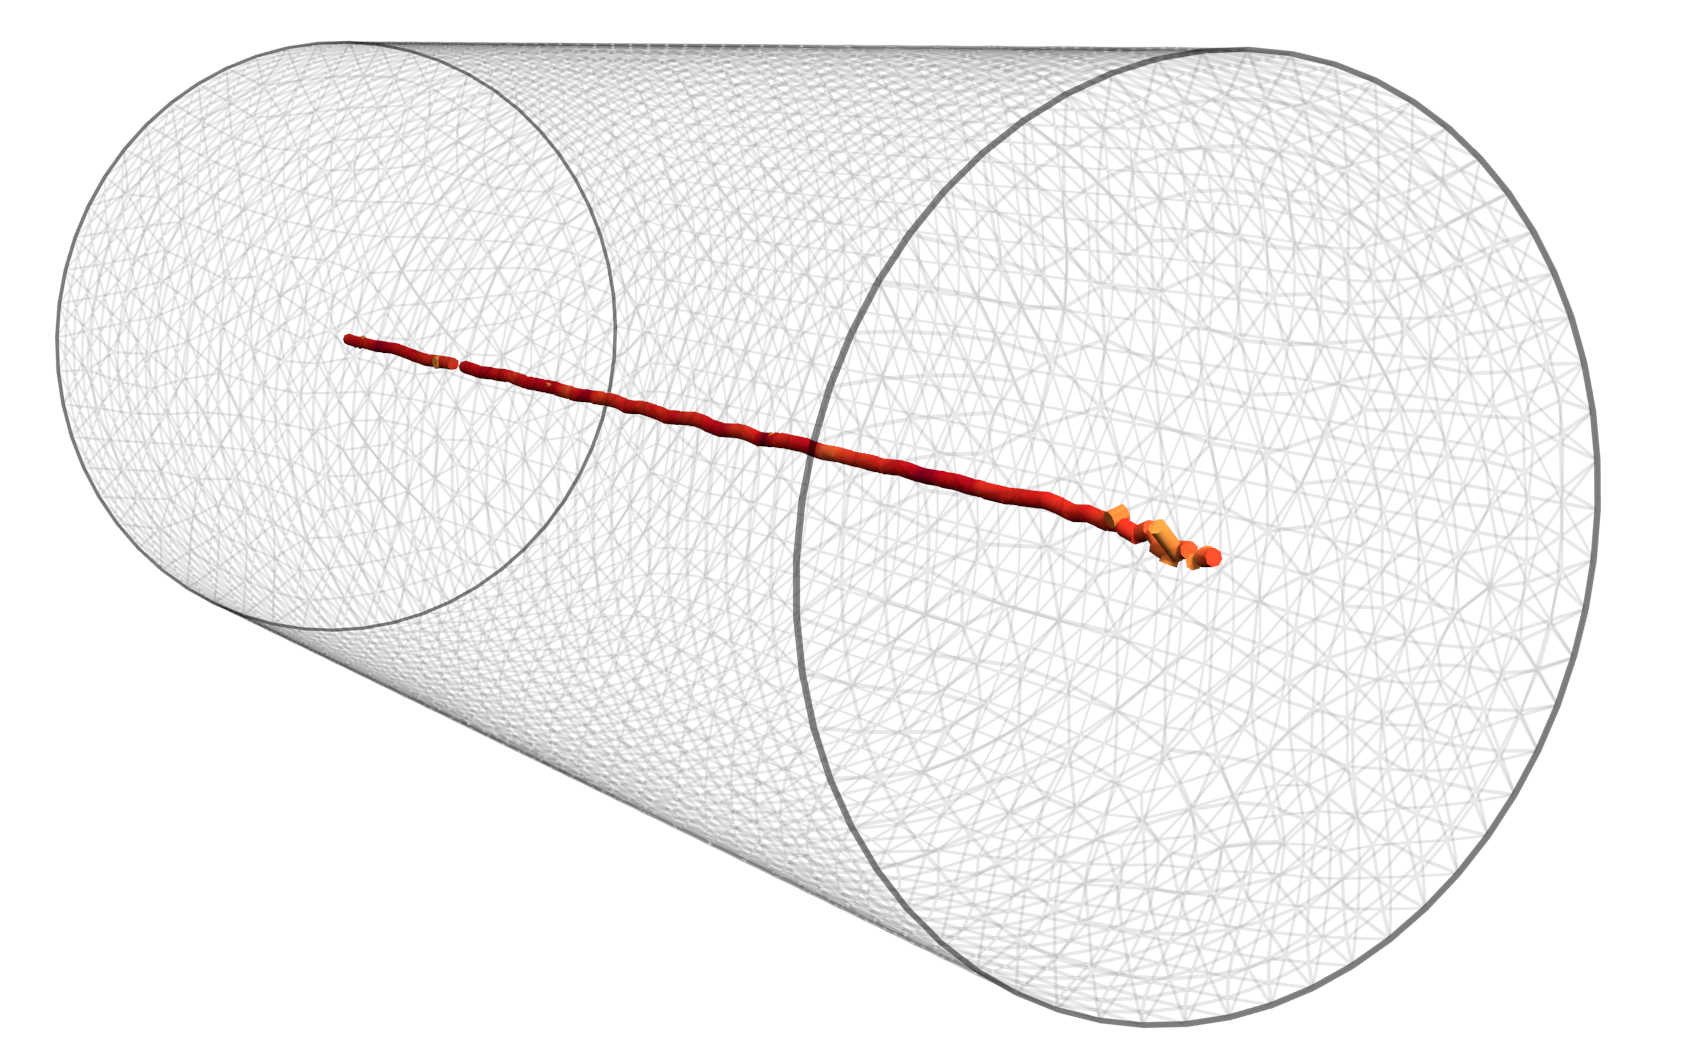
\includegraphics[width=0.45\figurewidth]{figures/cylinder_lines_m100}%
    };
    \node[anchor=south west] at (image1.south west) {\small $M = \num{100}$};

    \node[image, right=of image1] (image2)
    {
        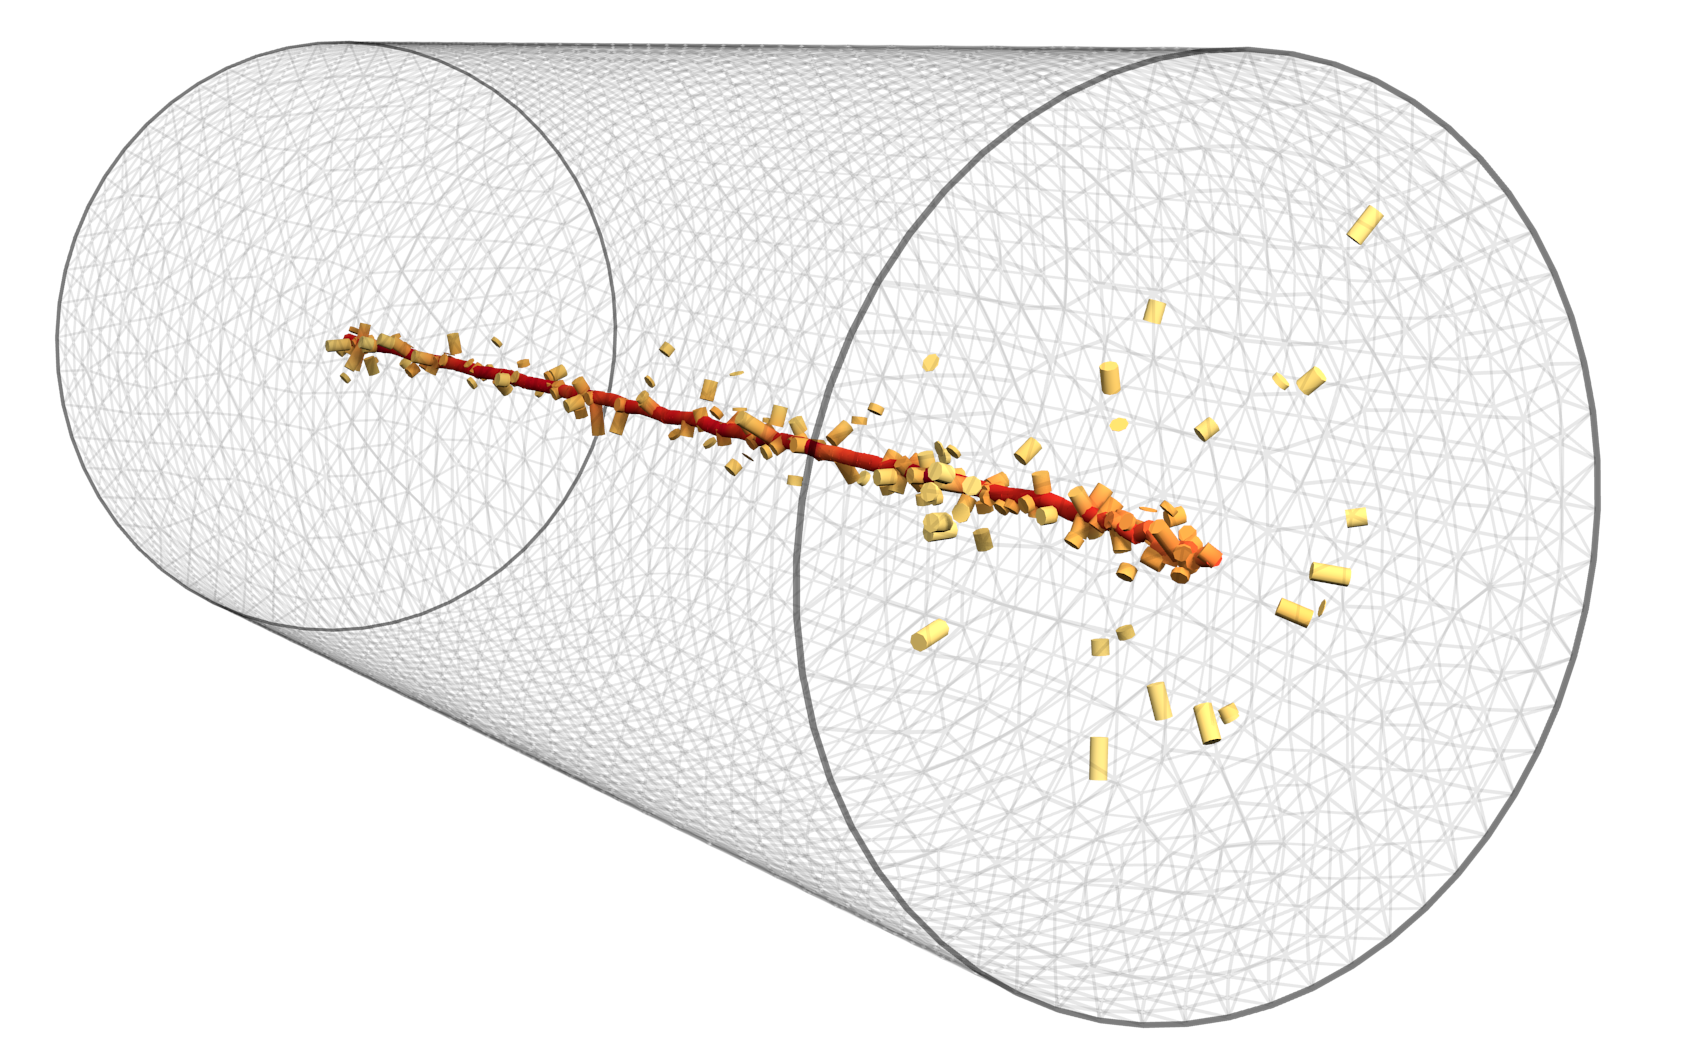
\includegraphics[width=0.45\figurewidth]{figures/cylinder_lines_m1000}%
    };
    \node[anchor=south west] at (image2.south west) {\small $M = \num{1000}$};

    \node[image, below=of image1, yshift=-0.1cm] (image3)
    {
        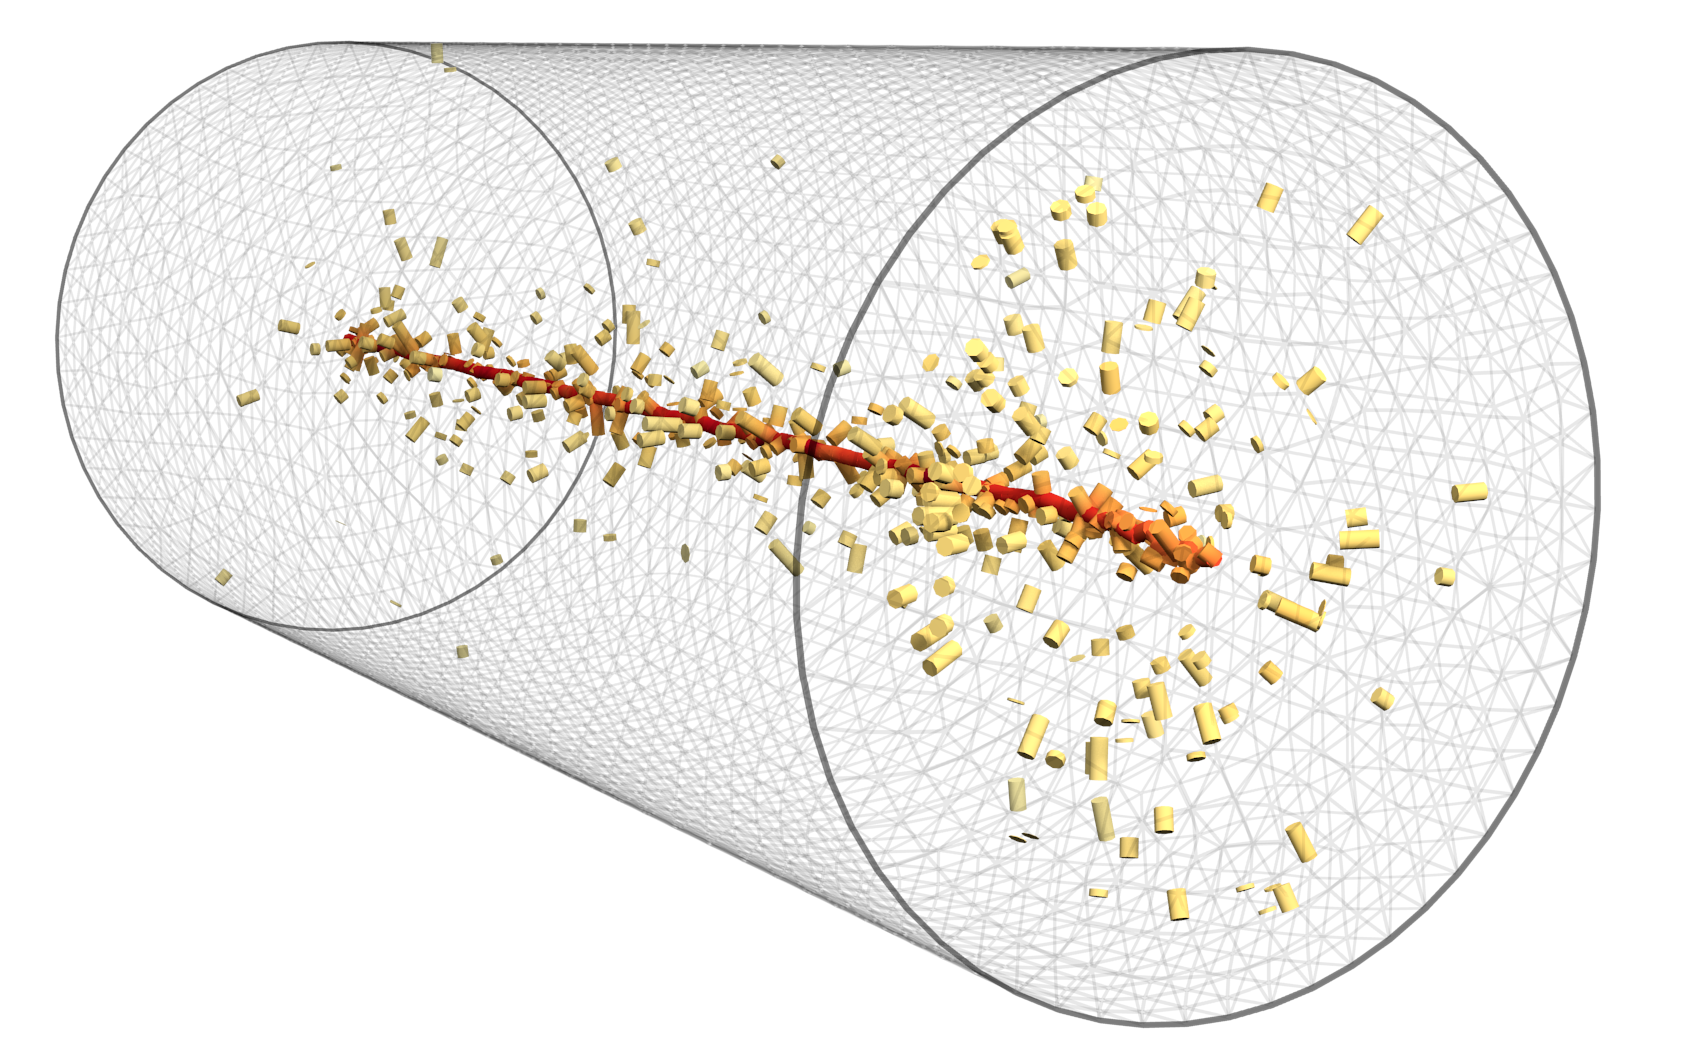
\includegraphics[width=0.45\figurewidth]{figures/cylinder_lines_m10000}%
    };
    \node[anchor=south west] at (image3.south west) {\small $M = \num{10000}$};

    \node[image, right=of image3] (image4)
    {
        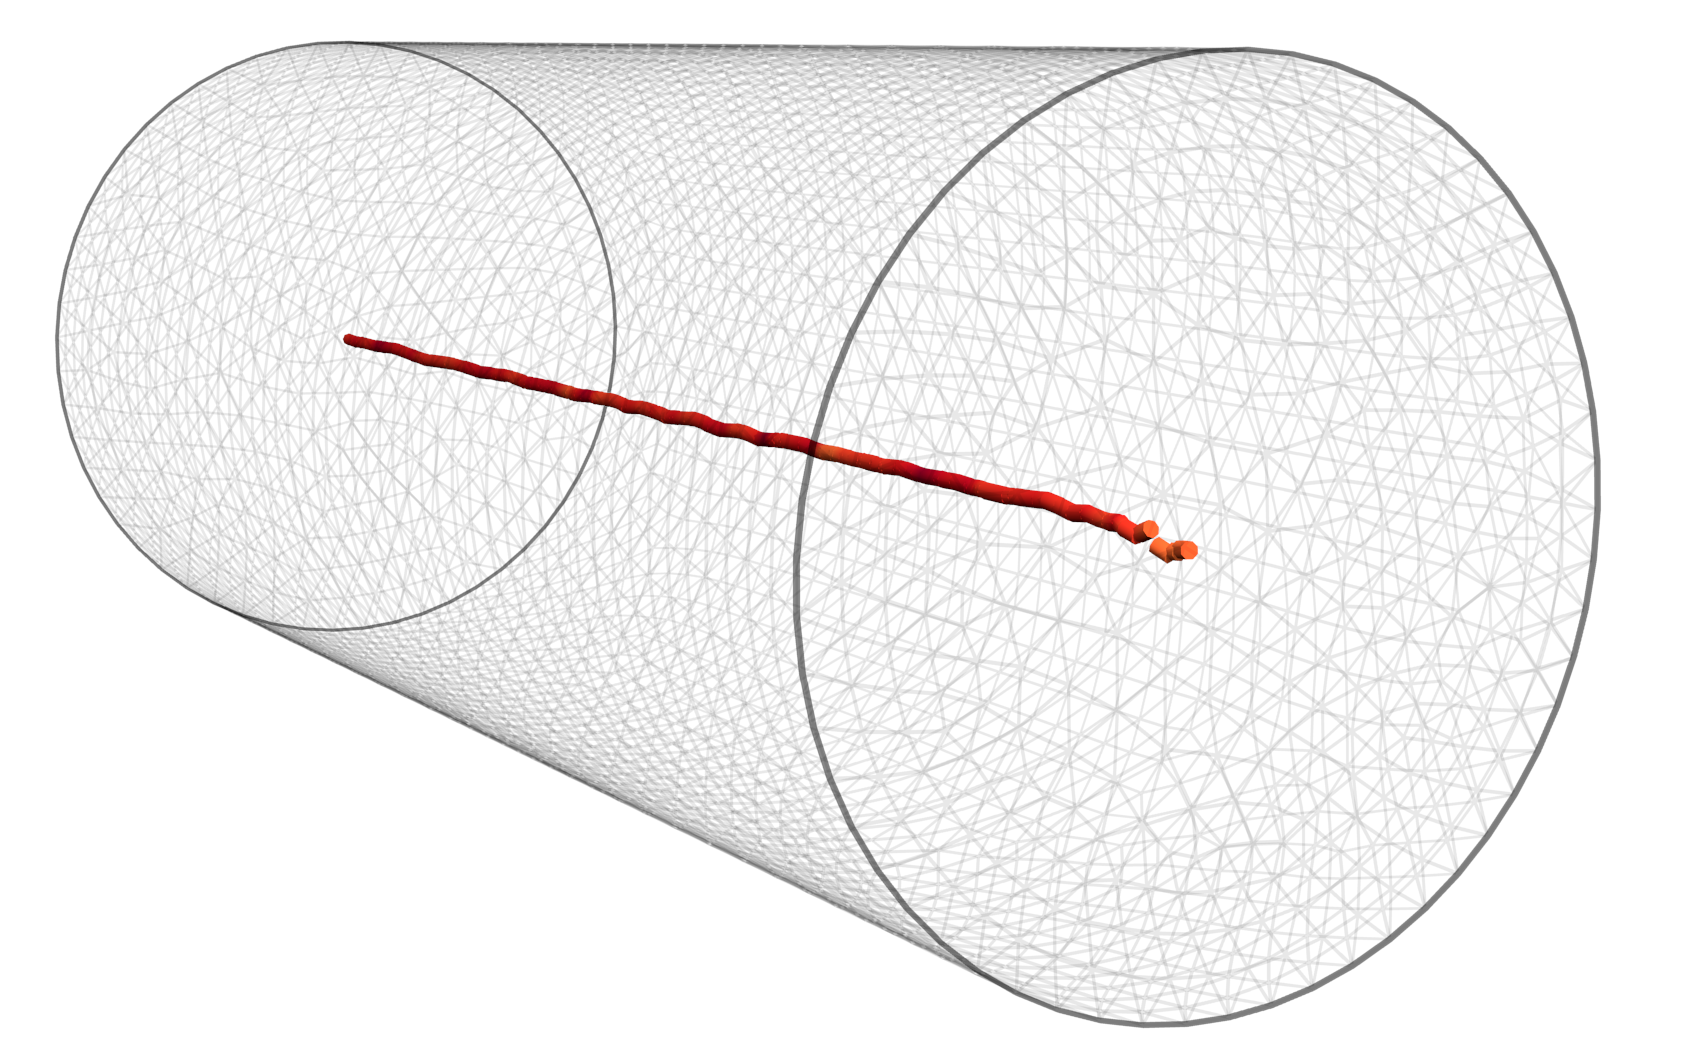
\includegraphics[width=0.45\figurewidth]{figures/cylinder_lines_filtered}%
    };
    \node[anchor=south west] at (image4.south west) {\small filtered};

    \node[anchor=west, xshift=-0.75cm] at (image4.north east){
        \begin{axis}[
        scale only axis,
        height=4cm,
        hide axis,
        domain=1:20,
        colorbar,
        colorbar/width=0.25cm,
        colormap name={rdoryl},
        point meta min=1, point meta max=20,
        colorbar style={
            title=$\log(s)$,
            scaled ticks=false,
            ytick={1, 20}
        }]
      \end{axis}
    };

\end{tikzpicture}
    \caption{Results of our algorithm on the Cylinder dataset for different
             choices of $M$. Increasing $M$ results in more numerically unstable
             lines being found. If we filter them out, the result is virtually
             identical.}
    \label{fig:unfiltered_lines}
\end{figure}
%
% subsection performance (end)
%
\subsection{Comparison with Degenerate Lines} % (fold)
\label{sub:comparison_with_degenerate_lines}
%
Tensor core lines are mathematically distinct from degenerate lines where two or
more eigenvalues are equal.
%
The criterion for finding tensor core lines is completely independent of the
eigenvalues of the tensor field.
%
However, when looking at our results in stress tensor fields, one might wonder
if tensor core lines coincide with degenerate lines in practice.
%
To investigate this, we extracted degenerate lines from our datasets using the
method presented by Zheng and Pang \cite{Zheng2004}.
%
In stress tensor fields, degenerate lines mark locations where no unique
principal directions of stress can be established.
%
We found that tensor core lines and degenerate lines sometimes coincide, but
neither is a subset of the other.
%
In the Crane dataset, degenerate lines are found near the center of the lower
diagonal rods, where we also find tensor core lines.
%
However, a lot of degenerate lines are also found in regions where no tensor
core lines are located.
%
In the Truck Bumper dataset, a degenerate line coincides with one of the two
most significant tensor core lines we find, but not the other one.
%
Closeups of both datasets are shown in~\autoref{fig:topo_comparison}.
%
In several datasets, such as the Cylinder and Handle, Zheng and Pang's method
fails to locate any degenerate lines at all.
%
\begin{figure}[t]
    \centering
    \setlength{\figurewidth}{0.8\textwidth}
    %
\begin{tikzpicture}[
    image/.style={inner sep=0, outer sep=0, node distance = 0 and 0},
    label/.style={anchor=north west, fill=white, font=\small, xshift=1mm, yshift=-1mm}
]

    \node[image, anchor=south west] (image1)
    {
        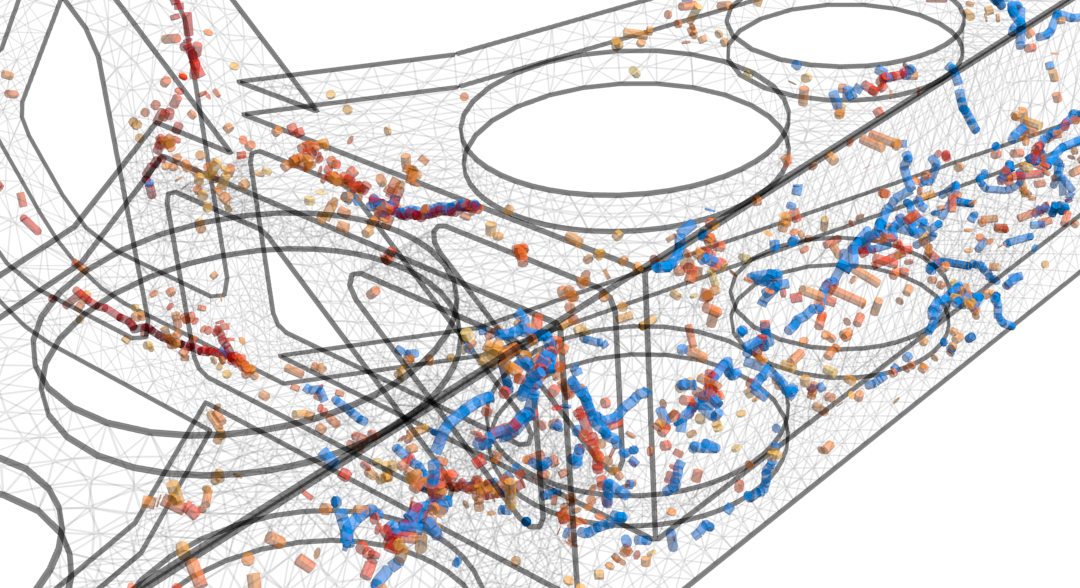
\includegraphics[width=\figurewidth]{figures/truck_bumper_topo_lines_detail2_slim}%
    };
    \begin{scope}[
        shift=(image1.south west), % origin is lower left corner
        x={($(image1.south east)-(image1.south west)$)}, % x axis is lower side
        y={($(image1.north west)-(image1.south west)$)}] % y axis is left side
        % \draw[help lines,xstep=.1,ystep=.1] (0,0) grid (1,1);
        % \foreach \x in {0,1,...,9} { \node [anchor=north] at (\x/10,0) {\scriptsize 0.\x}; }
        % \foreach \y in {0,1,...,9} { \node [anchor=east] at (0,\y/10) {\scriptsize 0.\y}; }
        \draw[red,very thick,rounded corners] (0.3,0.57) rectangle (0.47,0.68);
    \end{scope}
    \node[label] at (image1.north west) {\textsc{Truck Bumper}};

    \node[image, below=of image1, yshift=-0.2cm] (image2)
    {
        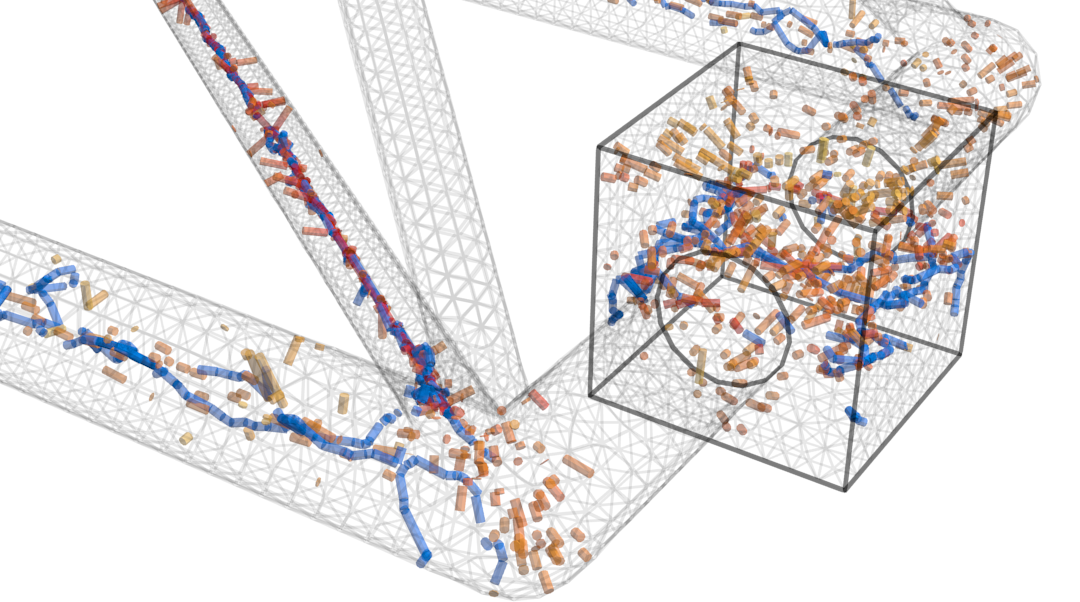
\includegraphics[width=\figurewidth]{figures/crane_topo_lines_detail1_slim}%
    };
    \begin{scope}[
        shift=(image2.south west), % origin is lower left corner
        x={($(image2.south east)-(image2.south west)$)}, % x axis is lower side
        y={($(image2.north west)-(image2.south west)$)}] % y axis is left side
        % \draw[help lines,xstep=.1,ystep=.1] (0,0) grid (1,1);
        % \foreach \x in {0,1,...,9} { \node [anchor=north] at (\x/10,0) {\scriptsize 0.\x}; }
        % \foreach \y in {0,1,...,9} { \node [anchor=east] at (0,\y/10) {\scriptsize 0.\y}; }
        \draw[mycolor4, very thick, rotate around={-57:(0.295, 0.66)}]
            (0.295, 0.66) ellipse (0.21 and 0.04);
    \end{scope}
    \node[label] at (image2.north west) {\textsc{Crane}};
\end{tikzpicture}
    \caption{Comparison of unfiltered tensor core lines (red/yellow) and
    degenerate tensor lines (blue) for the Truck Bumper (top) and Crane dataset
    (bottom). The red box marks the coincidence of a numerically stable tensor
    core line with a degenerate tensor line.}
    \label{fig:topo_comparison}
\end{figure}
%
% subsection comparison_with_degenerate_lines (end)
%
% section results (end)